%%%%%%%%%%%%%%%%%%%%%%%%%%%%%%%%%%%%%%%%%
% Oliver Lemon made minor edits (jan 2015)  to : 
% Masters/Doctoral Thesis 
% LaTeX Template
% Version 1.43 (17/5/14)
%
% This template has been downloaded from:
% http://www.LaTeXTemplates.com
%
% Original authors:
% Steven Gunn 
% http://users.ecs.soton.ac.uk/srg/softwaretools/document/templates/
% and
% Sunil Patel
% http://www.sunilpatel.co.uk/thesis-template/
%
% License:
% CC BY-NC-SA 3.0 (http://creativecommons.org/licenses/by-nc-sa/3.0/)
%
% Note:
% Make sure to edit document variables in the Thesis.cls file
%
%%%%%%%%%%%%%%%%%%%%%%%%%%%%%%%%%%%%%%%%%

%----------------------------------------------------------------------------------------
%	PACKAGES AND OTHER DOCUMENT CONFIGURATIONS
%----------------------------------------------------------------------------------------

\documentclass[10pt, oneside]{Thesis} % The default font size and one-sided printing (no margin offsets)

\graphicspath{{Pictures/}} % Specifies the directory where pictures are stored
\usepackage{ragged2e}
\usepackage[square,numbers]{natbib}
\bibliographystyle{unsrtnat}
\hypersetup{urlcolor=blue, colorlinks=true} % Colors hyperlinks in blue - change to black if annoying


\title{HWU CS Masters thesis template} % BUT you should use use " \title{\ttitle} " here instead to define the thesis title ! 
% \ttitle is defined in the file Thesis.cls 

\begin{document}

\frontmatter % Use roman page numbering style (i, ii, iii, iv...) for the pre-content pages

\setstretch{1.3} % Line spacing of 1.3

% Define the page headers using the FancyHdr package and set up for one-sided printing
\fancyhead{} % Clears all page headers and footers
\rhead{\thepage} % Sets the right side header to show the page number
\lhead{} % Clears the left side page header

\pagestyle{fancy} % Finally, use the "fancy" page style to implement the FancyHdr headers

\newcommand{\HRule}{\rule{\linewidth}{0.5mm}} % New command to make the lines in the title page

% PDF meta-data
\hypersetup{pdftitle={\ttitle}}
\hypersetup{pdfsubject=\subjectname}
\hypersetup{pdfauthor=\authornames}
\hypersetup{pdfkeywords=\keywordnames}

%----------------------------------------------------------------------------------------
%	TITLE PAGE
%----------------------------------------------------------------------------------------

\begin{titlepage}
\begin{center}
{\scshape\LARGE ASSAM UNIVERSITY \par}\vspace{1.5cm}

\HRule \\[0.4cm] % Horizontal line
{\huge \textbf{Segmentation and Classification of Brain Tumor in MRI Images}}\\[0.3cm] % Thesis title
\HRule \\[1.5cm] % Horizontal line

\large \textit{A report submitted in partial fulfilment of the requirements for the degree of \\ \textbf{ Bachelor of Technology}}\\[0.3cm] % University requirement text
\textit{in }\\ \textbf{Computer Science and Engineering}
%\groupname\\


 
\begin{minipage}[t]{0.8\textwidth}
\begin{center}
  \textbf{Submitted By:}\\
  \begin{flushleft}
  K.A. Moriom Sultana \hspace{3.0cm} 42-160081208 of 2016-17\\
  Anurag Kushawaha \hspace{3.4cm} 42-150068213 of 2015-16\\
  Rakesh Das \hspace{4.8cm} 42-150068224 of 2015-16\\ % Author name - remove the \href bracket to remove the link 
 \end{flushleft}
\end{center} \large


\end{minipage}
\\[0.8cm]
\begin{minipage}[t]{0.8\textwidth}
\begin{center} \large
\textbf{Under the guidance of:} \\
{Dr. Sudipta Roy}\\Professor\\Department of Computer Science and Engineering\\Dean\\Triguna Sen School of Technology
%\\
%Dean, Department of Computer Science and Engineering
 %\\ Supervisor name - remove the \href bracket to remove the link  
\end{center}
\end{minipage}\\[1cm]
 {

\includegraphics[width=3cm]{Logo.png} \\% University/department logo - uncomment to place it
Triguna Sen School of Tehnology\\ 
Department of Computer Science and Engineering\\ % Research group name and department name
Assam University, Silchar 788011 \\
\large 27th May, 2019}\\[1cm] % Date
\end{center}

\end{titlepage}

%----------------------------------------------------------------------------------------
%	DECLARATION PAGE
%	Your institution may give you a different text to place here
%----------------------------------------------------------------------------------------
\begin{center}
    
\includegraphics[width=4cm]{Logo.png} % University/department logo - uncomment to place it
 

\end{center}
\Declaration{

\addtocontents{toc}{\vspace{1em}} % Add a gap in the Contents, for aesthetics



 We, the undersigned, declare that this report titled, '\Brain Tumor Detection Using MRI Images' and the work presented in this report is our own. We confirm that this work submitted for assessment is our own and is expressed in our own words. Any uses made within it of the works of  other authors in any form (e.g., ideas, equations, figures, text,  tables, programs) are properly acknowledged at any point of their  use . To the best of our knowledge and belief, the same report has not been submitted either by us or by any other person for the award of any other degree or diploma of the university or other
institute of higher learning.

%\begin{itemize} 
%\item[\tiny{$\blacksquare$}] This work was done wholly or mainly while in candidature for a research degree at this University.
%\item[\tiny{$\blacksquare$}] Where any part of this thesis has previously been submitted for a degree or any other qualification at %this University or any other institution, this has been clearly stated.
%\item[\tiny{$\blacksquare$}] Where I have consulted the published work of others, this is always clearly attributed.
%\item[\tiny{$\blacksquare$}] Where I have quoted from the work of others, the source is always given. With the exception of such %quotations, this thesis is entirely my own work.
%\item[\tiny{$\blacksquare$}] I have acknowledged all main sources of help.
%\item[\tiny{$\blacksquare$}] Where the thesis is based on work done by myself jointly with others, I have made clear exactly what %was done by others and what I have contributed myself.\\
%\end{itemize}
 \vspace{2cm} 
K A Moriom Sultana (31420095)\\%(Name,Roll No and Signature)\\
\rule[1em]{40em}{0.5pt}\\ % This prints a line for the signature
Anurag Kushawaha (31420013) \\
\rule[1em]{40em}{0.5pt}\\
Rakesh Das (31420024)\\
\rule[1em]{40em}{0.5pt}\\
Date: 27th May 2019\\
\rule[1em]{20em}{0.5pt}\\ % This prints a line to write the date
Place: Silchar,Assam\\
\rule[1em]{20em}{0.5pt}\\
}

\clearpage % Start a new page

%-------------------------------------------------------------------------------

%-------------------------------------------------------------------------------
% CERTIFICATE PAGE
%
% Use the \Certificate command to print the Certificate in the document
%-------------------------------------------------------------------------------

\begin{center}

\includegraphics[width=3cm]{Logo.png}\\ % University/department logo - uncomment to place it
Department of Computer Science and Engineering \\
Assam University, Silchar-788003\\
\Certificate{
This is to certify that the report entitled \\ \textit{\Brain Tumor Detection Using MRI Images} \\ and submitted by \\ \textit{\textbf{\ K A Moriom Sultana\\Anurag Kushawaha\\Rakesh Das}} \\ to the Department of Computer Science and Engineering, Assam University, Silchar in partial fulfilment of the requirements for the the award of the Degree of\\ \textbf{Bachelor of Technology} \\ in \\ \textbf{Computer Science and Engineering} \\ is a bonafide record of the work carried out by them under my supervision.It is further certified that the candidates has  complied with all the formalities as per the requirements of \\Assam University.\\ \vspace{2cm}



\begin{flushleft}
 \rule[1em]{30em}{0.5pt}\\  \textbf{Dr.Sudipta Roy(Dean)}  \\ \vspace{1cm}
 \rule[1em]{30em}{0.5pt}\\ \textbf{Dr. Sunita Sarkar (Head of the Department)}  \\ \vspace{1cm}
\rule[1em]{30em}{0.5pt}\\ \textbf{External Examiner's Name \& Signature}  \\
\begin{flushright}
Date and Seal
\end{flushright}
\end{flushleft} \large








}
\end{center}
\clearpage








%----------------------------------------------------------------------------------------
%	QUOTATION PAGE
%----------------------------------------------------------------------------------------

% \pagestyle{empty} % No headers or footers for the following pages

% \null\vfill % Add some space to move the quote down the page a bit

% \textit{``You have to dream before your dreams come true."}

% \begin{flushright}
% Dr. A.P.J. Abdul Kalam
% \end{flushright}

% \vfill\vfill\vfill\vfill\vfill\vfill\null % Add some space at the bottom to position the quote just right

% \clearpage % Start a new page

%----------------------------------------------------------------------------------------
%	ABSTRACT PAGE
%----------------------------------------------------------------------------------------

\addtotoc{Abstract} % Add the "Abstract" page entry to the Contents

%\abstract{\addtocontents{toc}{\vspace{1em}} % Add a gap in the Contents, for aesthetics

 {\huge{\textit{Abstract}} \par}{\addtocontents{toc}{\vspace{1em}} 

Today’s recent medical imaging research faces the challenge of detecting brain tumor through Magnetic Resonance Images (MRI). Broadly, to produce images of soft tissue of human body, MRI images are used by experts. For brain tumor detection, image segmentation is required. Mechanizing this process is a tricky task because of the high diversity in the appearance of tumor tissues among different patients and in many cases similarity with the usual tissues.Physical segmentation of medical image by the radiologist is a monotonous and prolonged process. MRI is a highly developed medical imaging method providing rich information about the person soft-tissue structure. There are varied brain tumor recognition and segmentation methods to detect and segment a brain tumor from MRI images. This is well thought-out to be one of the most significant but tricky part of the process of detecting brain tumor. A variety of algorithms were developed for segmentation of MRI images by using different tools and methods. Alternatively this paper presents a comprehensive review of the methods and techniques used to detect brain tumor through MRI image.  
%The page is kept centered vertically so can expand into the blank space above the title too\ldots
%

\clearpage % Start a new page

%----------------------------------------------------------------------------------------
%	ACKNOWLEDGEMENTS
%----------------------------------------------------------------------------------------

\setstretch{1.3} % Reset the line-spacing to 1.3 for body text (if it has changed)

\acknowledgements{\addtocontents{toc}{\vspace{1em}} % Add a gap in the Contents, for aesthetics

I would like to express my thanks to the people who have helped me most throughout my project.

I am grateful to my mentor and guide Dr. Sudipta Roy for nonstop support for the project.

A special thank of mine goes to my friends who helped me out in completing the project, where they all exchanged their own interesting ideas, thoughts and made this possible to complete my project with all accurate information. I wish to thank my parents for their personal support or attention who inspired me to go my own way.
}
\clearpage % Start a new page

%----------------------------------------------------------------------------------------
%	LIST OF CONTENTS/FIGURES/TABLES PAGES
%----------------------------------------------------------------------------------------

\pagestyle{fancy} % The page style headers have been "empty" all this time, now use the "fancy" headers as defined before to bring them back

\lhead{\emph{Contents}} % Set the left side page header to "Contents"
\tableofcontents % Write out the Table of Contents

\lhead{\emph{List of Figures}} % Set the left side page header to "List of Figures"
\listoffigures % Write out the List of Figures

\lhead{\emph{List of Tables}} % Set the left side page header to "List of Tables"
\listoftables % Write out the List of Tables

%----------------------------------------------------------------------------------------
%	ABBREVIATIONS
%----------------------------------------------------------------------------------------

\clearpage % Start a new page

%\setstretch{1.5} % Set the line spacing to 1.5, this makes the following tables easier to read
%\vspace{0.5cm}
\lhead{\emph{Abbreviations}} % Set the left side page header to "Abbreviations"
\listofsymbols{ll} % Include a list of Abbreviations (a table of two columns)
{
\textbf{MRI} & \textbf{M}agnetic \textbf{R}esonance \textbf{I}mage \\
\textbf{CT} & \textbf{C}omputed \textbf{T}omography
\\
\textbf{EM} & \textbf{E}lectro \textbf{M}agnetic
\\
\textbf{MSER} & \textbf{M}aximally \textbf{S}table \textbf{E}xtremal \textbf{R}egions
\\
\textbf{FLAIR} & \textbf{F}luid \textbf{A}ttenuated \textbf{I}nversion \textbf{R}ecovery
\\
\textbf{DNN} & \textbf{D}eep \textbf{N}eural \textbf{N}etwork
\\
\textbf{CT} & \textbf{C}omputed \textbf{T}omography
\\
\textbf{CNN} & \textbf{C}onvolution \textbf{N}eural \textbf{N}etwork
\\
\textbf{PET} & \textbf{P}osition \textbf{E}mission \textbf{T}omography
\\
\textbf{MSE} & \textbf{M}ean \textbf{S}quared \textbf{E}rror
\\
\textbf{KNN} & \textbf{K} \textbf{N}earest \textbf{N}eighbors
\\
\textbf{ANN} & \textbf{A}rtificial \textbf{N}eural \textbf{N}etwork
\\
\textbf{GUI} & \textbf{G}raphic \textbf{U}ser \textbf{I}nterface
\\
\textbf{GLCM} & \textbf{G}ray \textbf{L}evel \textbf{C}o-occurrence \textbf{M}atrix
\\
\textbf{MLP} & \textbf{M}ulti \textbf{L}ayer
\textbf{P}erceptron
\\
\textbf{SVM}  &  \textbf{S}upport  \textbf{V}ector \textbf{M}achine
 \\
 \textbf{PNN}  &  \textbf{P}robablistic  \textbf{N}eural \textbf{N}etwork
\\
 \textbf{LM}  &  \textbf{L}evenberg  \textbf{M}arquart
\\
 \textbf{TP}  &  \textbf{T}rue  \textbf{P}ositive
\\
 \textbf{TN}  &  \textbf{T}rue  \textbf{N}egative
\\
 \textbf{FP}  &  \textbf{F}alse  \textbf{P}ositive
\\
 \textbf{FN}  &  \textbf{F}alse   \textbf{N}egative
\\
\textbf{PCA} & \textbf{P}rincipal \textbf{C}omponent \textbf{A}nalysis} \\
%\textbf{Acronym} & \textbf{W}hat (it) \textbf{S}tands \textbf{F}or \\
}

%----------------------------------------------------------------------------------------
%	PHYSICAL CONSTANTS/OTHER DEFINITIONS
%----------------------------------------------------------------------------------------

%\clearpage % Start a new page

%\lhead{\emph{Physical Constants}} % Set the left side page header to "Physical Constants"

%\listofconstants{lrcl} % Include a list of Physical Constants (a four column table)
%{
%Speed of Light & $c$ & $=$ & $2.997\ 924\ 58\times10^{8}\ \mbox{ms}^{-\mbox{s}}$ (exact)\\

%% Constant Name & Symbol & = & Constant Value (with units) \\
%}

%----------------------------------------------------------------------------------------
%	SYMBOLS
%----------------------------------------------------------------------------------------

\clearpage % Start a new page

%\lhead{\emph{Symbols}} % Set the left side page header to "Symbols"

%\listofnomenclature{lll} % Include a list of Symbols (a three column table)
%{
%$a$ & distance & m \\
%$P$ & power & W (Js$^{-1}$) \\
%% Symbol & Name & Unit \\

%& & \\ % Gap to separate the Roman symbols from the Greek

%$\omega$ & angular frequency & rads$^{-1}$ \\
% Symbol & Name & Unit \\
%}

%----------------------------------------------------------------------------------------
%	DEDICATION
%----------------------------------------------------------------------------------------

\setstretch{1.3} % Return the line spacing back to 1.3

\pagestyle{empty} % Page style needs to be empty for this page

%\dedicatory{For/Dedicated to/To my\ldots} % Dedication text

\addtocontents{toc}{\vspace{2em}} % Add a gap in the Contents, for aesthetics

%----------------------------------------------------------------------------------------
%	THESIS CONTENT - CHAPTERS
%----------------------------------------------------------------------------------------

\mainmatter % Begin numeric (1,2,3...) page numbering

\pagestyle{fancy} % Return the page headers back to the "fancy" style

% Include the chapters of the thesis as separate files from the Chapters folder
% Uncomment the lines as you write the chapters

% Chapter 1

\chapter{Introduction} % Main chapter title

\label{Chapter1} % For referencing the chapter elsewhere, use \ref{Chapter1} 

\lhead{Chapter 1. \emph{ Introduction }} % This is for the header on each page - perhaps a shortened title

%----------------------------------------------------------------------------------------
\section{Overview}
Healthcare sector is totally different from other industry. It is on high priority sector and people expect highest level of care and services regardless of cost. After the success of deep learning in other real-world application, it is also providing exciting solutions with good accuracy for medical imaging and is a key method for future applications in health sector. Brain is an organ that controls activities of all the parts of the body. Recognition of automated brain tumor in
Magnetic resonance imaging (MRI) is a difficult task due to complexity of size and location variability. In this thesis, statistical analysis morphological and thresholding techniques are proposed to process the images obtained by MRI for Tumor Detection from Brain MRI Images. 

In recent times, the introduction of information technology and e-health care system in the medical field helps clinical experts to provide effective diagnosis, treatment and monitoring of the disease for better health care to the patient.The most recent big advances in Magnetic Resonance Imaging (MRI) technology have been on the software side, enabling faster contrast scans. Magnetic resonance imaging (MRI) is a noninvasive medical test that helps physicians diagnose and treat medical conditions.

MRI uses a powerful magnetic field, radio frequency pulses and a computer to produce detailed pictures of organs, soft tissues, bone and virtually all other internal body structures. The images can then be examined on a computer monitor, transmitted electronically, printed or copied to a CD. MRI does not use ionizing radiation (x-rays). Detailed MR images allow physicians to evaluate various parts of the body and determine the presence of certain diseases.

In the literature review, there are many techniques and algorithms which were developed and implemented for image segmentation that are histogram based, edge-based, artificial neural network based methods, region-based methods (region growing, splitting and merging), physical model based approaches, and clustering methods (K-means clustering, Fuzzy C-means clustering), but still there is a necessity  to identify and develop an efficient and  fast technique for  medical image segmentation, because, all these techniques have their own advantages and limitations with reference to their  suitability, applicability, performance and computational time. 

Brain tumors are a solid neoplasm inside the skull. These tumors arise as a result of the uncontrolled and abnormal cell division. Usually they grow in the brain itself, but also grow in other places such as in lymphatic tissue, in blood vessels, in the cranial nerves, in the brain envelopes. Brain tumors can also grow as a result of the spread of cancers primarily located in other parts of the body. Classification of brain tumors depends on the tumor location, the type tissue which the tumor created, whether the tumor is malignant or benign, and other considerations. Also MRI can be performed on any individual ranging from adults to small children. Therefore, a large dataset is available to test the proposed methodology.

The difficulty in segmentation process is the selection of proper method for a particular kind of image dataset. There is no generally accepted technique for brain MRI image segmentation. In this paper, image segmentation by region based (Morphological operations) technique is implemented.Magnetic resonance imaging (MRI) is done for many reasons. It is used to find problems such as tumors, bleeding, injury, blood vessel diseases, or infection. MRI  also may be done to provide more information about a problem seen on an X-ray, ultrasound scan, or CT scan. Contrast material may be used during MRI to show abnormal tissue more clearly. 

Morphological operations also called Mathematical morphology are used to segment the MR images of brain. Morphology deals with the application of the concepts of the set theory to image processing and analysis. It is concerned with the study of structures and shapes from a general scientific perspective. Morphological operations are normally performed on the binary images which represent the pixel values either 0 or 1. The Morphological filters are basically nonlinear transformations that modify the geometric features of the images. The morphological operator or filter transform the original image into another image by the process of iteration with another image of a suitable size and shape referred to as structuring element [14].

\section{Problem Statement}
An accurate classification of human cancer, including its primary site, is important for better understanding of cancer and effective therapeutic strategies development. The available big data of somatic mutations provides a great opportunity to investigate cancer classification using machine learning. In this research primary sites classification using machine learning and somatic mutation data is proposed. Here, in this research the patterns exploration of 1,760,846 somatic mutations identified from 230,255 cancer patients along with gene function information using support vector machine is proposed. In this a multiclass classification experiment over the 17 tumor sites using the gene symbol, somatic mutation, chromosome, and gene functional pathway as predictors for 6,751 subjects is to be performed. Adding the information of mutation and chromosome will improve the result. Among the predictable primary tumor sites, the prediction of five primary sites (large intestine, liver, skin, pancreas, and lung) could achieve the performance with more in F-measure. expected outcome of this research is that more accurate result will be generated for Detection and Classification of cancer cells in MRI Images.

\section{MRI Contrasts}
Magnetic resonance imaging (MRI) is commonly used in medical image for analysis of brain tumors. MRI is a non-invasive system, which can be utilized alongside with other imaging modalities, such as computed tomography (CT), positron emission tomography (PET) to give accurate data for brain tumor structure. However, using these systems alongside MRI is expensive and, in some of the case, can be invasive (e.g. PET). Therefore, different MR that are non-invasive and image both structure and functions are mostly used for brain imaging. MRI machines themselves come with different configurations and produce images with varying intensities. This makes tumor detection a difficult task when different MRI configurations (such as magnetic field strength 1.5, 3 or 7 Tesla) and the acquisition protocol (field of view value, voxel resolution, gradient strength, b0 value, etc.) are used. These configurations have different intensity values across voxels, which result in the same tumorous cells may have different grayscale values when pictured in different hospitals. MRI can show different tissue contrasts through different pulse sequences, making it an adaptable and widely used imaging technique for visualizing regions of interest in the human brain. MRI modalities are combined to produce multi-modal images giving more information about irregular shaped tumors, which are difficult to localize with a single modality. These modalities include T1-weighted MRI (T1), T1-weighted MRI with contrast enhancement (T1c), T2-weighted MRI (T2) and T2-weighted MRI with fluid attenuated inversion recovery (T2-Flair). This multi-modal data contains information that can be used for tumor segmentation with significant improvement in performance. Figure 1 shows an axial slice of the four standard sequences for a glioma patient including manually drawn tumor regions. T1-weighting is the most commonly used sequence for the structural analysis; it also allows for an easy annotation of the healthy tissues. In T1-weighted contrast-enhanced images (gadolinium-DTPA), the tumor borders appear brighter because the contrast agent accumulates there due to the disruption of the blood–brain barrier in the proliferative tumor region. In this sequence, the necrotic and the active tumor region can be distinguished easily. In T2-weighted MRI, the edema region, which surrounds the tumor, appears bright. T2FLAIR (FLAIR) is a special sequence, which helps in separating the edema region from the cerebrospinal fluid (CSF) because the free water signal is suppressed. The radiological definition of the tumor margins in the clinical context are often manually determined by the radiologist on the T2 and post-gadolinium T1 images by thresholding boundaries between T2 hyperintense/T1 contrast-enhanced lesions and the surrounding healthy tissue to define the outer margins of a tumor.

\begin{figure}[htbp]
      \centering
      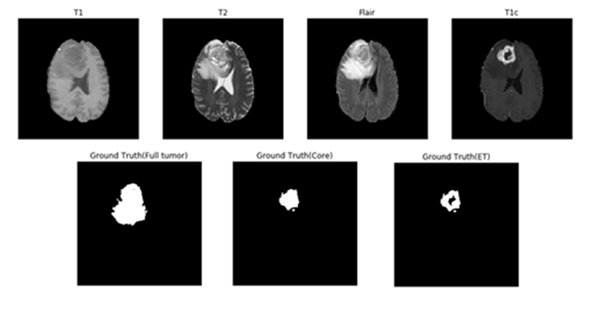
\includegraphics[scale=0.43]{Figures/MRI.png}
      \caption[Dataset Overview]{One axial slice of an MR image of a high-grade glioma patient. From left to right in row 1: T1-weighted image, T2-weighted image, T2-FLAIR-weighted image T1-weighted image with contrast enhancement. In row 2, showing the three sub-region ground truth labeled by exports}
      \label{fig:MRI_slice}
 \end{figure}

%-----------------------------------------------------------------------------------------------------------------------------------------------------------------------------------------------------------------------------------------------------
% Chapter Template

\chapter{Machine Learning} % Main chapter title

\label{Chapter7} % Change X to a consecutive number; for referencing this chapter elsewhere, use \ref{ChapterX}

\lhead{Chapter 2. \emph{Machine Learning}} % Change X to a consecutive number; this is for the header on each page - perhaps a shortened title

%----------------------------------------------------------------------------------------
%	SECTION 1
%----------------------------------------------------------------------------------------

\section{Definition}

Machine Learning is the field of study that gives computers the capability to learn without being explicitly programmed. ML is one of the most exciting technologies that one would have ever come across. As it is evident from the name, it gives the computer that which makes it more similar to humans: The ability to learn. Machine learning is actively being used today, perhaps in many more places than one would expect.

\begin{itemize}
\item Traditional Programming: Data and program is run on the computer to produce the output.
\item Machine Learning: Data and output is run on the computer to create a program. This program can be used in traditional programming.
\end{itemize}
\begin{figure}[htbp]
    \centering
	    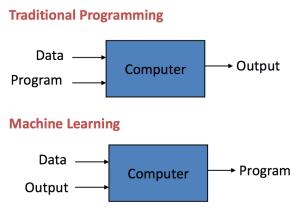
\includegraphics[scale=0.5]{Figures/tl_ml.png}
		    %\rule{10em}{0.5pt}
        \caption[Traditional programming vs Machine Learning]{Traditional programming vs Machine Learning}
	    \label{fig:Traditional programming vs Machine Learning}
\end{figure}
 Machine learning is like farming or gardening. Seeds is the algorithms, nutrients is the data, the gardener is you and plants is the programs.
\clearpage
\section{Types of Machine Learning}

At a high-level, machine learning is simply the study of teaching a computer program or algorithm how to progressively improve upon a set task that it is given. On the research-side of things, machine learning can be viewed through the lens of theoretical and mathematical modeling of how this process works. However, more practically it is the study of how to build applications that exhibit this iterative improvement. There are many ways to frame this idea, but largely there are three major recognized categories:
\begin{enumerate}
    \item Supervised learning
    \item Unsupervised learning
    \item Reinforcement learning
\end{enumerate}

\begin{figure}[htbp]
    \centering
	    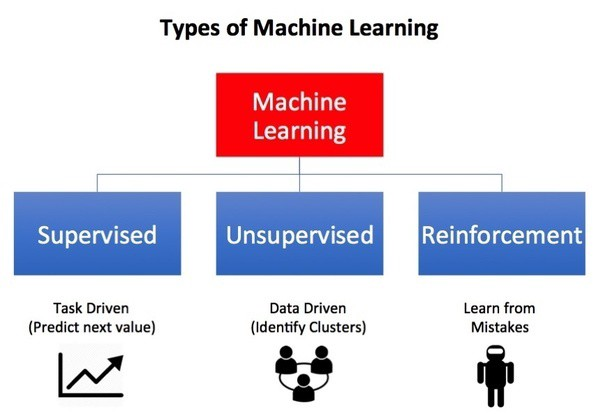
\includegraphics[scale=0.3]{Figures/ml_types.jpg}
		    %\rule{10em}{0.5pt}
        \caption[Types of Machine Learning]{Types of Machine Learning}
	    \label{fig:Traditional programming vs Machine Learning}
\end{figure}

\subsection{Supervised Learning}

Supervised learning is the most popular paradigm for machine learning. It is the easiest to understand and the simplest to implement.\\
Given data in the form of examples with labels, we can feed a learning algorithm these example-label pairs one by one, allowing the algorithm to predict the label for each example, and giving it feedback as to whether it predicted the right answer or not. Over time, the algorithm will learn to approximate the exact nature of the relationship between examples and their labels. When fully-trained, the supervised learning algorithm will be able to observe a new, never-before-seen example and predict a good label for it.

\begin{figure}[htbp]
    \centering
	    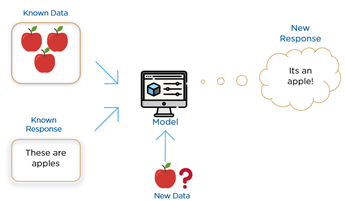
\includegraphics[scale=0.4]{Figures/supervised.png}
		    %\rule{10em}{0.5pt}
        \caption[Supervised Learning]{Supervised Learning}
	    \label{fig:Supervised Learning}
\end{figure}

Supervised Learning uses two types of techniques:

\begin{itemize}
    \item Classification:
        Classification is the process of predicting the class of given data points. Classes are sometimes called as targets/ labels or categories. Classification predictive modeling is the task of approximating a mapping function (f) from input variables (X) to discrete output variables (y).

        For example, spam detection in email service providers can be identified as a classification problem. This is s binary classification since there are only 2 classes as spam and not spam. A classifier utilizes some training data to understand how given input variables relate to the class. In this case, known spam and non-spam emails have to be used as the training data. When the classifier is trained accurately, it can be used to detect an unknown email.

        Classification belongs to the category of supervised learning where the targets also provided with the input data. There are many applications in classification in many domains such as in credit approval, medical diagnosis, target marketing etc.

        There are two types of learners in classification as lazy learners and eager learners.
        \begin{enumerate}
            \item Lazy learners: Lazy learners simply store the training data and wait until a testing data appear. When it does, classification is conducted based on the most related data in the stored training data. Compared to eager learners, lazy learners have less training time but more time in predicting.

            \textit {Ex. k-nearest neighbor, Case-based reasoning}
    
            \item Eager learners: Eager learners construct a classification model based on the given training data before receiving data for classification. It must be able to commit to a single hypothesis that covers the entire instance space. Due to the model construction, eager learners take a long time for train and less time to predict.

            \textit{Ex. Decision Tree, Naive Bayes, Artificial Neural Networks}
    
        \end{enumerate}
        Classification Algorithms:\\
        There is a lot of classification algorithms available now but it is not possible to conclude which one is superior to other. It depends on the application and nature of available data set. For example, if the classes are linearly separable, the linear classifiers like Logistic regression, Fisher’s linear discriminant can outperform sophisticated models and vice versa.
        \begin{itemize}
            \item Decision Tree:
                
                Decision tree builds classification or regression models in the form of a tree structure. It utilizes an if-then rule set which is mutually exclusive and exhaustive for classification. The rules are learned sequentially using the training data one at a time. Each time a rule is learned, the tuples covered by the rules are removed. This process is continued on the training set until meeting a termination condition.
            
            \begin{figure}[htbp]
                \centering
	            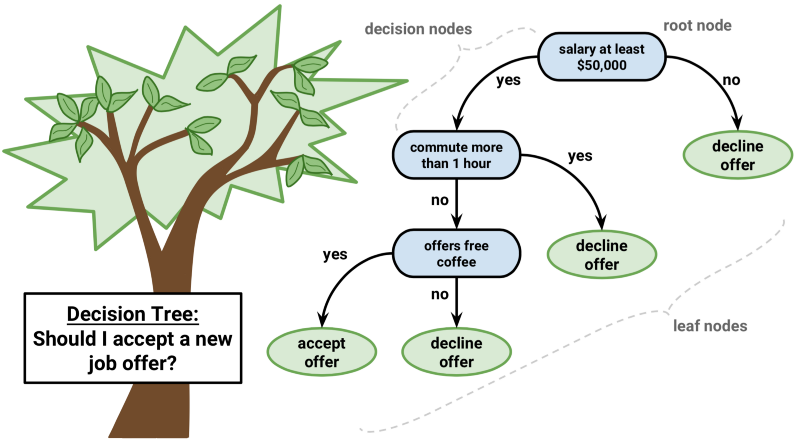
\includegraphics[scale=0.3]{Figures/decision_tree.png}
		        %\rule{10em}{0.5pt}
                \caption[Decision Tree]{Decision Tree}
	            \label{fig:Decision Tree}
                \end{figure}

                The tree is constructed in a top-down recursive divide-and-conquer manner. All the attributes should be categorical. Otherwise, they should be discretized in advance. Attributes in the top of the tree have more impact towards in the classification and they are identified using the information gain concept.

                A decision tree can be easily over-fitted generating too many branches and may reflect anomalies due to noise or outliers. An over-fitted model has a very poor performance on the unseen data even though it gives an impressive performance on training data. This can be avoided by pre-pruning which halts tree construction early or post-pruning which removes branches from the fully grown tree.

        \item Naive Bayes:
                Naive Bayes is a probabilistic classifier inspired by the Bayes theorem under a simple assumption which is the attributes are conditionally independent.\\
                    \begin{figure}[htbp]
                        \centering
	                    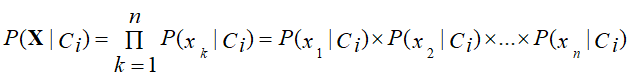
\includegraphics[scale=0.5]{Figures/naive_bayes.png}
		                %\rule{10em}{0.5pt}
                        \caption[Naive Bayes]{Naive Bayes}
	                    \label{fig:Naive Bayes}
                    \end{figure}
                The classification is conducted by deriving the maximum posterior which is the maximal P(Ci|X) with the above assumption applying to Bayes theorem. This assumption greatly reduces the computational cost by only counting the class distribution. Even though the assumption is not valid in most cases since the attributes are dependent, surprisingly Naive Bayes has able to perform impressively.

                Naive Bayes is a very simple algorithm to implement and good results have obtained in most cases. It can be easily scalable to larger datasets since it takes linear time, rather than by expensive iterative approximation as used for many other types of classifiers.

                Naive Bayes can suffer from a problem called the zero probability problem. When the conditional probability is zero for a particular attribute, it fails to give a valid prediction. This needs to be fixed explicitly using a Laplacian estimator.
                
        \item Artificial Neural Networks:
                Artificial Neural Network is a set of connected input/output units where each connection has a weight associated with it started by psychologists and neurobiologists to develop and test computational analogs of neurons. During the learning phase, the network learns by adjusting the weights so as to be able to predict the correct class label of the input tuples.

                \begin{figure}[htbp]
                    \centering
	                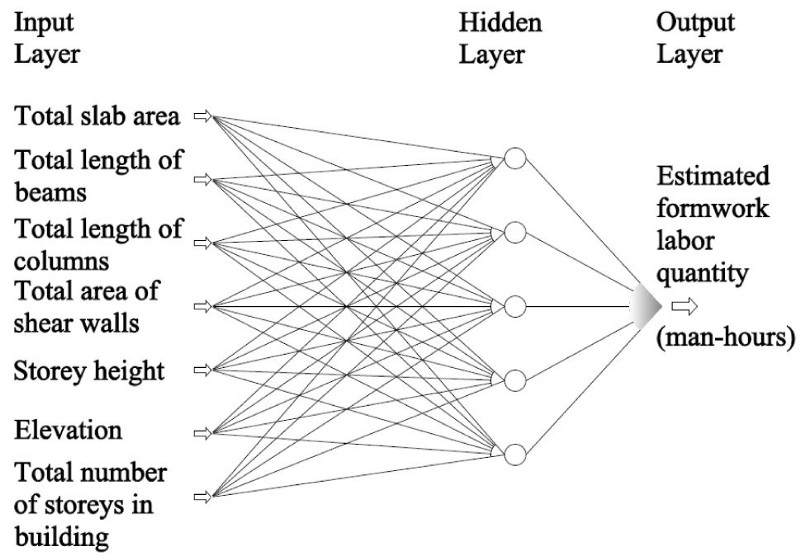
\includegraphics[scale=0.3]{Figures/ann.jpeg}
		            %\rule{10em}{0.5pt}
                    \caption[Artificial Neural Network Design]{Artificial Neural Network Design}
	                \label{fig:Naive Bayes}
                \end{figure}
                
                There are many network architectures available now like Feed-forward, Convolutional, Recurrent etc. The appropriate architecture depends on the application of the model. For most cases feed-forward models give reasonably accurate results and especially for image processing applications, convolutional networks perform better.

                There can be multiple hidden layers in the model depending on the complexity of the function which is going to be mapped by the model. Having more hidden layers will enable to model complex relationships such as deep neural networks.

                However, when there are many hidden layers, it takes a lot of time to train and adjust wights. The other disadvantage of is the poor interpretability of model compared to other models like Decision Trees due to the unknown symbolic meaning behind the learned weights.

                But Artificial Neural Networks have performed impressively in most of the real world applications. It is high tolerance to noisy data and able to classify untrained patterns. Usually, Artificial Neural Networks perform better with continuous-valued inputs and outputs.

        \item k-Nearest Neighbor (KNN):
                \begin{figure}[htbp]
                    \centering
	                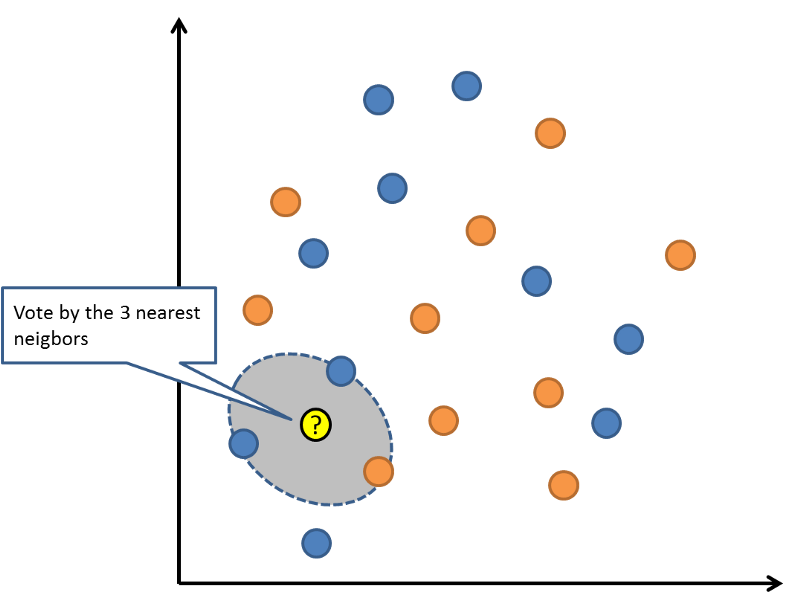
\includegraphics[scale=0.3]{Figures/knn.png}
		            %\rule{10em}{0.5pt}
                    \caption[k-Nearest Neighbor]{k-Nearest Neighbor}
	                \label{fig:Naive Bayes}
                \end{figure}
        
                k-Nearest Neighbor is a lazy learning algorithm which stores all instances correspond to training data points in n-dimensional space. When an unknown discrete data is received, it analyzes the closest k number of instances saved (nearest neighbors)and returns the most common class as the prediction and for real-valued data it returns the mean of k nearest neighbors.

                In the distance-weighted nearest neighbor algorithm, it weights the contribution of each of the k neighbors according to their distance using the following query giving greater weight to the closest neighbors.

                \begin{figure}[htbp]
                    \centering
	                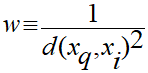
\includegraphics[scale=0.5]{Figures/knn2.png}
		            %\rule{10em}{0.5pt}
                    \caption[Distance calculating query]{Distance calculating query}
	                \label{fig:Naive Bayes}
                \end{figure}
        \end{itemize}
    \item Regression:
                \begin{figure}[htbp]
                    \centering
	                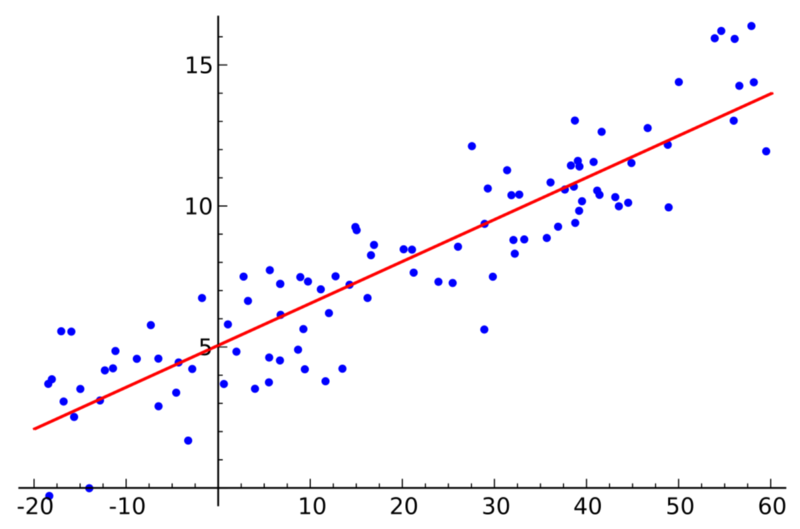
\includegraphics[scale=0.4]{Figures/linear_r.png}
		            %\rule{10em}{0.5pt}
                    \caption[Distance calculating query]{Distance calculating query}
	                \label{fig:Naive Bayes}
                \end{figure}
    
        Simple linear regression is a type of regression analysis where the number of independent variables is one and there is a linear relationship between the independent(x) and dependent(y) variable. The red line in the above graph is referred to as the best fit straight line. Based on the given data points, we try to plot a line that models the points the best. The line can be modelled based on the linear equation shown below.
    
                \begin{figure}[htbp]
                    \centering
	                
\includegraphics[scale=0.8]{Figures/linear_r1.png}
		            %\rule{10em}{0.5pt}
                \end{figure}
                
        The motive of the linear regression algorithm is to find the best values for a0 and a1. Before moving on to the algorithm, let’s have a look at two important concepts you must know to better understand linear regression.
        
        \clearpage
        Cost Function: The cost function helps us to figure out the best possible values for a0 and a1 which would provide the best fit line for the data points. Since we want the best values for a0 and a1, we convert this search problem into a minimization problem where we would like to minimize the error between the predicted value and the actual value.
        
                \begin{figure}[htbp]
                    \centering
	                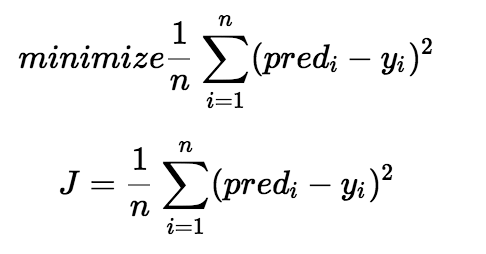
\includegraphics[scale=0.5]{Figures/costfn.png}
		            %\rule{10em}{0.5pt}
		            \caption[Minimization and Cost Function]{Minimization and Cost Function}
	                \label{fig:Minimization and Cost Function}
                \end{figure}
                
        We choose the above function to minimize. The difference between the predicted values and ground truth measures the error difference. We square the error difference and sum over all data points and divide that value by the total number of data points. This provides the average squared error over all the data points. Therefore, this cost function is also known as the Mean Squared Error(MSE) function. Now, using this MSE function we are going to change the values of a0 and a1 such that the MSE value settles at the minima.
        
        Gradient Descent: The next important concept needed to understand linear regression is gradient descent. Gradient descent is a method of updating a0 and a1 to reduce the cost function(MSE). The idea is that we start with some values for a0 and a1 and then we change these values iteratively to reduce the cost. Gradient descent helps us on how to change the values.

                \begin{figure}[htbp]
                    \centering
	                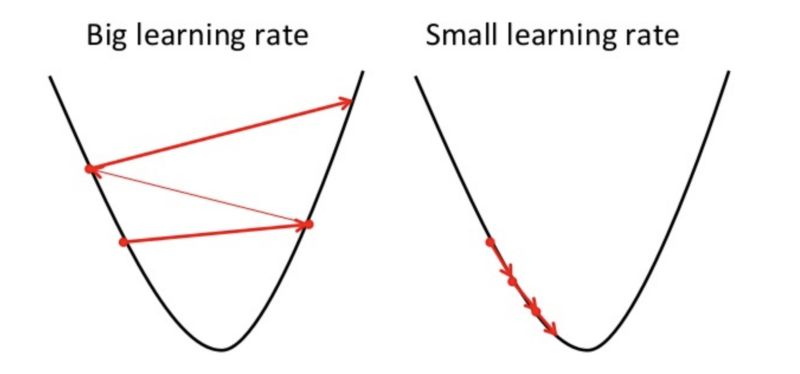
\includegraphics[scale=0.4]{Figures/lrate.png}
		            %\rule{10em}{0.5pt}
		            \caption[Learning Rate]{Learning Rate}
	                \label{fig:Learning Rate}
                \end{figure}
        To draw an analogy, imagine a pit in the shape of U and you are standing at the topmost point in the pit and your objective is to reach the bottom of the pit. There is a catch, you can only take a discrete number of steps to reach the bottom. If you decide to take one step at a time you would eventually reach the bottom of the pit but this would take a longer time. If you choose to take longer steps each time, you would reach sooner but, there is a chance that you could overshoot the bottom of the pit and not exactly at the bottom. In the gradient descent algorithm, the number of steps you take is the learning rate. This decides on how fast the algorithm converges to the minima.
    
\end{itemize}
\subsection{Unsupervised Learning}
    Unsupervised Learning is a class of Machine Learning techniques to find the patterns in data. The data given to unsupervised algorithm are not labelled, which means only the input variables(X) are given with no corresponding output variables. In unsupervised learning, the algorithms are left to themselves to discover interesting structures in the data.
% Chapter 2 

\chapter{Dataset} % Main chapter title

\label{Chapter2} % For referencing the chapter elsewhere, use \ref{Chapter2} 

\lhead{Chapter 2. \emph{ Dataset }} % This is for the header on each page - perhaps a shortened title

%-----------------------------------------------------------------
BraTS(Brain Tumor Segementation has always been focusing on the evaluation of state-of-the-art methods for the segmentation of brain tumors in multimodal magnetic resonance imaging (MRI) scans. BraTS utilizes multi-institutional pre-operative MRI scans and focuses on the segmentation of intrinsically heterogeneous (in appearance, shape, and histology) brain tumors, namely gliomas. Furthemore, to pinpoint the clinical relevance of this segmentation task, BraTS also focuses on the prediction of patient overall survival, via integrative analyses of radiomic features and machine learning algorithms.

    \begin{figure}[h!]
        \centering
        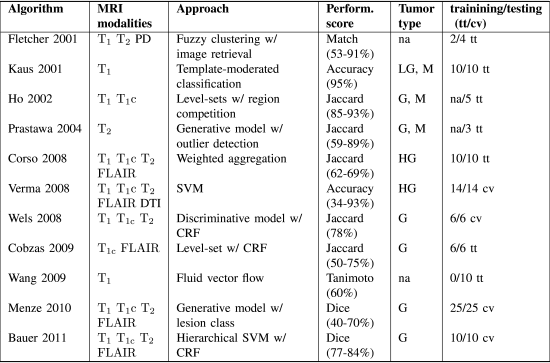
\includegraphics[scale=0.5]{Figures/dataset1.png}
        \caption[Dataset Description With Approaches]{Table I Data sets, MR image modalities, evaluation scores, and even tumor types used for self-reported performances in the brain tumor image segmentation literature differ widely. Shown Is a selection of algorithms discussed here and in [7]. Tumor type Is defined as g—glioma (unspecified), hg—high-grade glioma, lg—low-grade glioma, m—meningioma; “na” indicates that No information Is reported. When available the number of training and testing datasets Is reported, along with the testing mechanism: tt—separate training and testing datasets, cv—cross-validation}
        \label{fig:my_label}
    \end{figure}

   
\section{BraTS Dataset Annotations}
    
    BraTS images are available in .mha/nii(3d) format which we convert them to 2D images for deep learning processing. \\
    
    \begin{figure}[h!]
        \centering
        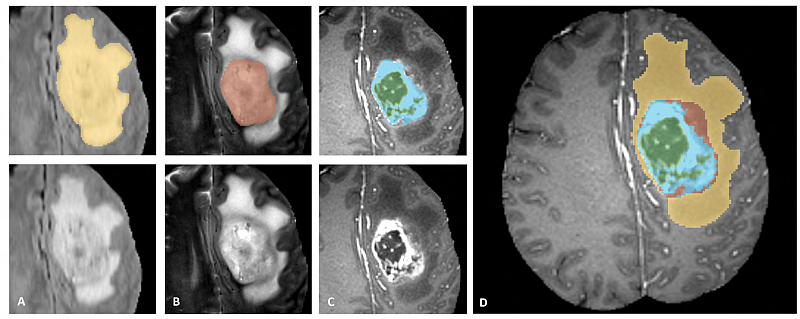
\includegraphics[scale=0.5]{Figures/BraTS_Tumors.png}
        \caption[BraTS Dataset Annotations]{Manual annotation through expert raters. Shown are image patches with the tumor structures that are annotated in the different modalities (top left) and the final labels for the whole dataset (right). Image patches show from left to right: the whole tumor visible in FLAIR (a), the tumor core visible in t2 (b), the enhancing tumor structures visible in t1c (blue), surrounding the cystic/necrotic components of the core (green) (c). Segmentations are combined to generate the final labels of the tumor structures (d): edema (yellow), non-enhancing solid core (red), necrotic/cystic core (green), enhancing core(blue)}
        \label{fig:BraTS_Dataset}
    \end{figure}
 
 

   
 \begin{table}[h!]
  \centering
  \caption{Types of brain MRI images}
    \begin{tabular}{|p{4cm}|p{3cm}|p{3cm}|p{3cm}|p{3cm}|}
       \hline
         \textbf{T1} & \textbf{T1c} & \textbf{T2} & \textbf{Flair} & \textbf{GT}\\
            \hline
            T1-weighted MRI & T1-enhanced weighted MRI & T2-weighted MRI & fluid-attenuated inversion-recovery MRI & Ground Truth\\
            \hline
        image contrast is based predominantly on the T1 (longgitudinal) relaxation time of tissue; tissue with short T1 relaxation time appears brighter & many tumors show signal enhancement after administration of contrast agent  & image contrast is based predominantly on the T2 (transverse) relaxation time of tissue; tissue with long T2 relaxation time appears brighter & bright signal of the CSF (cerebrospinal fluid) is suppressed which allows a better detection of small hyperintense lesions &  Actual region where the tumor is present \\
        \hline
            \end{tabular}
            
            \label{tab:my_label}
        \end{table}  
    
    
    
     
% Chapter 3

\chapter{Literature Survey} % Main chapter title

\label{Chapter3} % For referencing the chapter elsewhere, use \ref{Chapter3} 

\lhead{Chapter 3. \emph{ Literature Survey }} % This is for the header on each page - perhaps a shortened title

%-----------------------------------------------------------------

  \section{Bina Thomas and P K Nizar Banu \cite{ref1}}
  
  Bina Thomas and P K Nizar Banu,  in 2018 They used two image processing techniques  Median Filter and Gaussian Filter. Median filter is used to remove noise from an image and Gaussian Filter is used for blurring the image and sharpening the image.And this paper used different segmentation methods Watershed Segmentation and Gray level threshold segmentation and Canny edge detection and they used KNN(K nearest neighbors) algorithm they got the accuracy of 92.35\%.
  
  \section{Hussna Elnoor Mohammed Abdalla and M Y Esmail \cite{ref2}}
  
  Hussna Elnoor Mohammed Abdalla and M Y Esmail[2] in 2018 in this paper used Theshold segmentation by applied mean gray level method and  Morphological  operation and for classification they used Artificial Neural Network(ANN) and they got the best result with auccuracy 99\% and all result of this study step by step were presented in Graphic User Interface(GUI).
  
  \section{Hao Dong and  et al. \cite{ref3}}
  
  Hao Dong et al.[3] in 2017  in this paper they used U-net based deep neural networks and it is solving the brain tumor segmentation problem.The proposed method makes it possible to generate a patient-specific brain tumor segmentation model without manual interference, and this potentially enables objective lesion assessment for clinical tasks such as diagnosis, treatment planning and patient monitoring. In this paper FCN gives faster result(detect normal and abnormal tissues)
  
  \section{ Shubhangi S.Veer et al. \cite{ref4}}
  
   Shubhangi S.Veer et al.[4] in 2015 in this paper for Image processing they used the Median Filter and for feature extraction used Wavelet transformation and used different classifier that is MLP(Multi-Layer Parception),PCA(Principal Component Analysis),SVM(Support Vector Machine),PNN(Probablistic Neural Network).Among all the classifier MLP gives highest accuracy of 99\%.
   
   \section{Aqhsa Q.Syed and et al \cite{ref5}}
   
   Aqhsa Q.Syed et al.[5] in 2014 in this paper they used  used   Water-shed operation and Thresholding Segmentaion for segmenting tumor region and used MLP classification. It segments the tumor region  from the    Input    image and Multi-Layer Perception   Neural Network  is  used  to detect the image as Normal  Image for Normal  Brain  MRI input.

 
   \section{Nitish Zulpe and et al \cite{ref6}}
   
   Nitish Zulpe et al.[6] in 2012 in this paper they used GLCM for feature extraction and applied two layered feed forward Neural Network. This paper classify the 4 different classes of tumor i.e Astrocytoma, Meningioma, Sarcoma, Malastatic bron chogenic carcimoma. All the MRI slices collected from the WBA and after preprocessing the GLCM textural features used to train the feed forward neural network with Levenberg Marquart (LM) nonlinear optimization algorithm which gives the better recognition rate of 97.5\%. And this work will assist the physician to make the final decision for the further treatment.
  

\section{Comprehensive View}
\begin{table}[h!]
   \centering
    \begin{tabular}{|l|p{3cm}|p{3cm}|p{3cm}|p{3cm}|}
         \hline
        
    \textbf{YEAR} & \textbf{PAPER} &  \textbf{AUTHORS} &  \textbf{PROPOSED MODEL} & \textbf{ACCURACY RATE}\\
        
      \hline
      
     2018 & Brain Tumor Segmentation and Detection using MRI images & Bina Thomas and P K Nizar Banu  & Image Processing- Median Filter, Gaussian Filter Segmentation Method- Watershed Segmentation and Gray level threshold segmentation and Canny Edge Detection Classifier- Use KNN classification & 92.35\%  \\

    \hline
    
    2018 & Brain tumor Detection by using Artificial Neural Network(ANN) &  Hussna Elnoor Mohammed Abdalla and M Y Esmail  & This paper use theshold segmentation by applied mean gray level method and Morphological operation and for classification they used ANN  &    99\% \\

   \hline
   
   2017  & Automatic Brain tumor Detection and Segmentation using U-Net Based fully Convolutional Networks & Hao Dong et al. & Ihis paper used U-net based deep neural networks and it is solving the brain tumor segmentation problem & FCN gives faster result(detect normal and abnormal tissues)\\
   
   \hline
   
   2015  & Brain tumor Classifiication using Artificial Neural Network on MRI images & Shubhangi S.Veer and Pradeep M.Patil & For Image Processing they used  Median Filter for  Feature extraction-Wavelet transformation is been used and for  classification they used MLP,PCA,SVM,PNN & Among all the classifier MLP give highest accuracy of 99\% \\
        
  \hline
   
   2014  & Detection of Tumor in MRI images using Artificial Neural Network & Aqhsa Q.Syed and K. Narayanan & In this paper they used Watershed operation and Thresholding Segmentaion for segmenting tumor region and used MLP classification &  It segments the tumor region from the Input image and Multi-Layer Perception Neural Network is used to detect the image as Normal Image for Normal Brain MRI input \\

  \hline
 
  
  
  2012  & GLCM Textural Features for Brain Tumor Classification & Nitish Zulpe and Vrushsen Pawar & They used GLCM for feature extraction and applied to two layered Feed forward Neural Network   &   97.5\% \\
  
  \hline
  
  
   \end{tabular}
    \caption{Comprehensive View of Literature Survey}
    \label{tab:my_label}
 \end{table}
% Chapter 4

\chapter{Proposed Methodology} % Main chapter title

\label{Chapter4} % For referencing the chapter elsewhere, use \ref{Chapter4} 

\lhead{Chapter 4. \emph{ Proposed Methodology }} % This is for the header on each page - perhaps a shortened title

%-----------------------------------------------------------------------
In the previous chapter, we have discussed about the various machine learning techniques that are generally used  for Segmentation and Classification of Brain Tumor from MRI Images. We  have  used  some  of  these  techniques  on  our  dataset and  then  we  have  applied  our  model  on  the  dataset  to  compare  their  accuracy.   Before  these techniques are applied we have followed a few steps to process the data to remove null values and handle missing data from the dataset, this process is termed as data preprocessing.

This describes the materials, the source from which the brain image data collected and the algorithms for brain MRI segmentation and feature extraction. The methodology proposed includes application on brain MRI images of 256 × 256, 512 × 512 pixel size on dataset. It is converted into gray scale for further enhancement. The following discussion deals with implementation of algorithm.

Proposed method having following important blocks they are
\begin{enumerate}
    \item Pre-processing
    \item Patch Extraction
    \item Patch Pre-processing
    \item Feature Extraction
    \item CNN Training & Testing
    \item Performance
\end{enumerate}

The main Objective of this project is to accurately segment the brain abnormal portion by using the conventional neural network. A Convolutional Neural Network is used to segment the brain abnormal image by performing testing and training separately. To measure Sensitivity analysis includes true positive (TP), true negative (TN), false positive (FP), false negative (FN) etc. Pre-processing includes the removal of noise or unwanted distortion from the input image. It can help to increase the quality of the performance. Next step is to convert the image into patches or blocks to perform further operations. As we know we are using the neural network, we have to perform training as well as testing phases separately. For performing NNT training features should be extracted to learn neural network. Sensitivity analysis is used for performance anal


% \begin{figure}[h!]
%     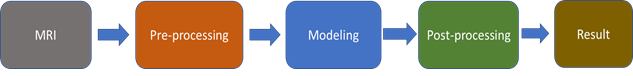
\includegraphics[scale=0.8]{Figures/p_model.png}
%     \caption{Proposed Methodoloy steps}
%     \label{fig:p_methodology}
% \end{figure}

\section{Pre-processing}
Preprocessing is one of the important steps in the image processing. In this work, mainly the preprocessing is done to perform the skull removal operation. By the combination of thresholding an morphological operation like dilation and erosion it is performed. A potential confounder in various image analysis tasks in the presence of a low-frequency intensity non-uniformity present in the image data also known as bias, in homogeneity, illumination non-uniformity, or gain field. 
N4ITK method is applied to MRI images to correct bias field distortion. MRI images are altered by the bias field distortion. However, this is not enough to ensure that the intensity distribution of a tissue type is in a similar intensity scale across different subjects for the same MRI sequence, which is an explicit or implicit assumption in most segmentation methods In fact, it can vary even if the image of the same patient is acquired in the same scanner in different time points, or in the presence of a pathology So, to make the contrast and intensity ranges more similar across patients and acquisitions, apply the intensity normalization a two-step method wherein all images (independent of patients and the specific brand of the MR scanner used) can be transformed in such a way that for the same protocol and body region, in the transformed images similar intensities will have similar tissue meaning.
In this intensity normalization method, a set of intensity landmarks are learned for each sequence from the training set and are chosen for each MRI sequence as described in represents the intensity at the percentile.

After training, the intensity normalization is accomplished by linearly transforming the original intensities between two landmarks into the corresponding learned landmarks. In this way, the histogram of each sequence is more similar across subjects. After normalizing the MRI images, we compute the mean intensity value and standard deviation across all training patches extracted for each sequence. Then, we normalize the patches on each sequence to have zero mean and unit variance.


    \subsection{Train/Test Split}
    The data we use is usually split into training data and test data. The training set contains a known output and the model learns on this data in order to be generalized to other data later on. We have the test dataset (or subset) in order to test our model’s prediction on this subset. The proportions generally used is 70\% in training and 30\% in testing data.  The training set and test set is divided into two parts x and y.

      \begin{figure}[h!]
        \centering
         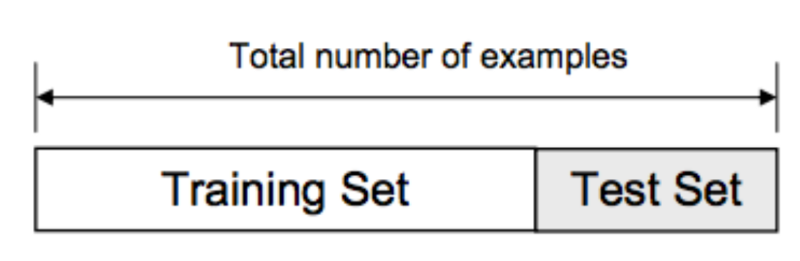
\includegraphics[scale=0.3]{Figures/split.png}
        \caption{Train/Test Split}
      \end{figure}
      
      \begin{itemize}
          \item Overfitting: 
          Overfitting means that model we trained has trained “too well” and is now, well, fit too closely to the training dataset. This usually happens when the model is too complex (i.e. too many features/variables compared to the number of observations). This model will be very accurate on the training data but will probably be very not accurate on untrained or new data. It is because this model is not generalized (or not AS generalized), meaning you can generalize the results and can’t make any inferences on other data, which is, ultimately, what you are trying to do. Basically, when this happens, the model learns or describes the “noise” in the training data instead of the actual relationships between variables in the data. This noise, obviously, isn’t part in of any new dataset, and cannot be applied to it.
          
          \item Underfitting: 
          In contrast to overfitting, when a model is underfitted, it means that the model does not fit the training data and therefore misses the trends in the data. It also means the model cannot be generalized to new data. As you probably guessed (or figured out!), this is usually the result of a very simple model (not enough predictors/independent variables). It could also happen when, for example, we fit a linear model (like linear regression) to data that is not linear. It almost goes without saying that this model will have poor predictive ability (on training data and can’t be generalized to other data)
      \end{itemize}
      
      \begin{figure}[h!]
        \centering
         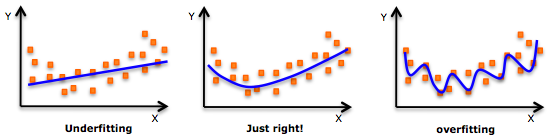
\includegraphics[scale=0.5]{Figures/over_under.png}
        \caption{An example of overfitting, underfitting and a balanced model}
      \end{figure}
      
      \subsection{Patch Extraction & Patch Pre-Processing}
      
    In patch extraction step, the images are converted into small blocks of size3x3. By converting into the patch, we can get more local information which can help to determine the tumor portion of the image. In this work, sliding windowing technique is used to extract the pixel blocks. By using sliding window more accurate information about the region we can estimate. In patch preprocessing the blocks will be converted into an array to find out the features of the local region.      
  
  
  
%   \begin{figure}
%       \centering
%       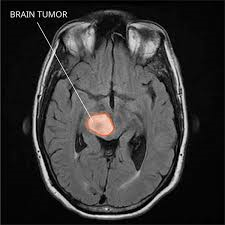
\includegraphics{Chapters/glioma.png}
%       \caption{Glioma}
%       \label{fig:my_label}
%   \end{figure}
%   \begin{figure}
%       \centering
%       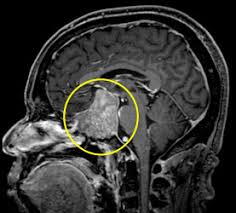
\includegraphics{Chapters/pituitary.png}
%      \caption{Pituitary}
%       \label{fig:my_label}
%   \end{figure}
    %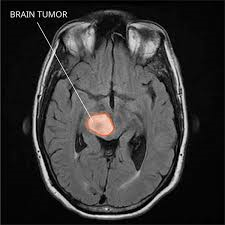
\includegraphics{Chapters/glioma.png}
   % \caption{Glioma}
    %\label{fig:my_label}
    
    %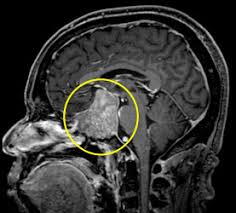
\includegraphics{Chapters/pituitary.png}
   %\caption{Pituitary}
    %\label{fig:my_label}
  %\end{figure}
%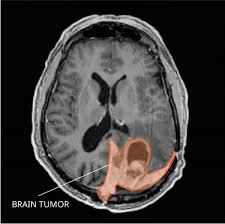
\includegraphics{Chapters/meningioma.png}
%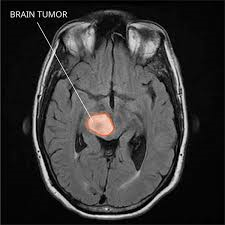
\includegraphics{Chapters/glioma.png}\\


\subsection{Image Segmentation}

The segmentation is a process where the image is partitioned into different regions. Let an entire region of image be represented by S. Segmentation process can be viewed as partition of S into p subregions like S1, S2, S3, …Sp. Certain conditions has to satisfied such as the segmentation must be intact; that is each and every pixel should be within the region, every points in the regions should be connected in some sense, regions should be disjoint, etc.

\subsection{Region growing}

Region growing is grouping of pixels or subregions into larger regions based on certain criteria. The main aim was to select a ‘seed’ points and attach each of these seed to those neighboring pixels having identical properties to grow region. A set of seeds was taken as input within the image and marked the objects to be segmented. The region grows iteratively by estimating all unallocated neighboring pixels of the region. The similarity was the measure of difference between pixel’s intensity value and the region’s mean, δ. The pixel with the smallest difference measured this way was allocated to the respective region. This was continued until all pixels were allocated to a region. Seeded region growing requires seeds as additional input. The results depend on the selection of seeds. The measurement was based on mean value of the pixel intensity. The image gets segmented; this image was used to identify the desired tumor region.

\section{Morphological Operation}

    Watershed transformation additionally called, as watershed method is an effective mathematical morphological tool for the image segmentation. It is more prevalent in the fields like biomedical and medical image processing, and computer vision. In topography, watershed means the edge that partitions area drained by diverse river system. If image is viewed as geological landscape, the watershed lines find out boundaries which separate image regions. The watershed transform figures catchment basins and ridge lines (otherwise called watershed lines), where catchment basins relating to image regions and ridge lines identifying with region boundaries. Segmentation by watershed embodies many of the concepts of the three techniques such as threshold based, edge based and region based segmentation.
    
    Watershed algorithms based on watershed transformation have mainly two classes. The first class contains the flooding based watershed algorithms and it is a traditional approach where as the second class contains rain falling based watershed algorithms. Many algorithms have been proposed in both classes but connected components based watershed algorithm shows very  good performance compared to all others. It comes under the rain falling based watershed algorithm approach. It gives very good segmentation results, and meets the criteria of less computational complexity.
    \newpage
    The steps for the operations are as follows:
  
    \begin{figure}[h!]
        \centering
            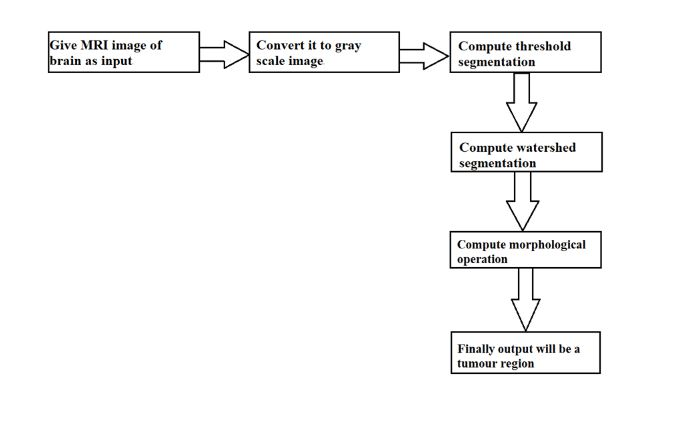
\includegraphics[scale=0.5]{Figures/water.png}
            \caption{Steps for Watershed & Morphological operation}
            \label{fig:my_label}
     \end{figure}
    
   
   \begin{enumerate}
       \item Give MRI image of brain as input
            Load the first MRI from the dataset. fig.4.6, shows the original image from which the tumor has to be detected  
        
            \begin{figure}[h!]
                 \centering
                 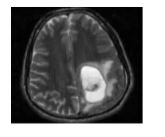
\includegraphics[scale=0.5]{Figures/11.png}
                 \caption{MRI Image}
                 \label{fig:my_label}
           \end{figure}
        \item Convert it to gray scale image
            The original image contains some RGB value. It has to be converted
            \begin{figure}[h!]
                \centering
                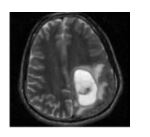
\includegraphics[scale=0.5]{Chapters/12.png}
                \caption{RGB to Gray converted image}
                \label{fig:RGB to Gray converted image}
            \end{figure}
        \item Compute threshold segmentation
            Threshold segmentation is one of the simplest segmentation systems. The input gray scale image is changed into a binary image.
            \begin{figure}[h!]
                \centering
                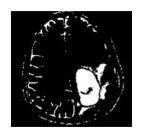
\includegraphics[scale=0.5]{Figures/13.png}
                \caption{Binary image}
                \label{fig:Binary image}
            \end{figure}
        \item Compute watershed segmentation
            Pixels falling under comparative intensities are assembled together. It is a decent segmentation system for separating a image to partition a tumor from the image. 
            After changing over the image in the binary format, some morphological operations are applied on it. The motivation behind the morphological operator is to discrete the tumor part of the image.
        \item Finally output will be a tumour region
        The fig. 5.7 shows the final extracted brain tumor
            \begin{figure}[h!]
                \centering
                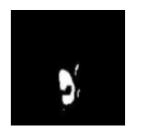
\includegraphics[scale=0.5]{Figures/14.png}
                \caption[Segmented Tumor Mask]{Segmented Tumor Mask}
                \label{fig:Segmented Tumor Mask}
            \end{figure}
   
   \end{enumerate}
 
\section{Feature Extraction}
It is the process of collecting higher-level information of an image such as shape, texture, color, and contrast.  It is used effectively to improve the accuracy of diagnosis system by selecting prominent features.

The statistics feature formula for features we have used are as follows:

\begin{enumerate}
    \item Mean (M): The mean of an image is calculated by adding all the pixel values of an image divided by the total number of pixels in an image.
    \item Standard Deviation (SD):  The standard deviation is the second central moment describing probability distribution of an observed population and can serve as a measure of in homogeneity. A higher value indicates better intensity level and high contrast of edges of an image.
    \item Entropy (E): Entropy is calculated to characterize the randomness of the textural image and is defined as corresponding states of intensity level which individual pixels can adapt. It is used in the quantitative analysis and evaluation image details, the entropy value is used as it provides better comparison of the image details.
    \item Energy (En): Energy can be defined as the quantifiable amount of the extent of pixel pair repetitions.
    \item Skewness ($S_k$): Skewness is a measure of symmetry or the lack of symmetry. The skewness of a random variable $X$ is denoted as $S_k(X)$.
    \item Kurtosis ($K_u_r_t$): The shape of a random variable’s probability distribution is described by the parameter called Kurtosis. For the random variable $X$, the Kurtosis is denoted as $K_u_r_t(X)$
    \item RMS(Root Mean Square): It is another way of calculating mean for set of pixels
    \item Variance: It is a measurement of the spread between pixels in an Image. The square root of variance is the standard deviation (σ).
\end{enumerate}

\section{Classification}
   
   Here we used many type of machine learning algorithm to
   classify the MRI of brain tumor and compare their performing, they are SVM, Decision tree, Naive Bayes, MLP, Logistic Regression.
  
\subsection{SVM}

  “Support Vector Machine” (SVM) is a supervised machine learning algorithm which can be used for both classification or regression challenges. However,  it is mostly used in classification problems. In this algorithm, we plot each data item as a point in n-dimensional space (where n is number of features you have) with the value of each feature being the value of a particular coordinate. Then, we perform classification by finding the hyper-plane that differentiate the two classes very well.
  
  
  \begin{figure}[h!]
  \centering
    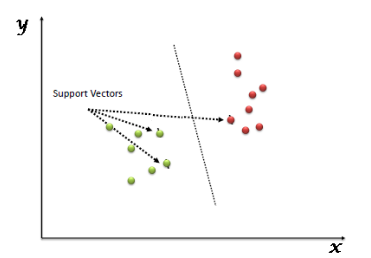
\includegraphics[scale=0.5]{Figures/svm11.png}
    \caption[SVM]{SVM}
    \label{fig:my_label}
  \end{figure}
  
  Support Vectors are simply the co-ordinates of individual observation. Support Vector Machine is a frontier which best segregates the two classes (hyper-plane/line).
  
  \subsubsection{How it Works}
  
  Above, we got accustomed to the process of segregating the two classes with a hyper-plane. Now the burning question is “How can we identify the right hyper-plane?”.
  
    \begin{enumerate}
        \item Identify the right hyper-plane(Scenario-1)
        Here, we  have three hyper-planes (A,B and C). Now, identify the right hyper-plane to classify star and circle.
            
        You need to remember a thumb rule to identify the right hyper-plane: “Select the hyper-plane which segregates the two classes better”. In this scenario, hyper-plane “B” has excellently performed this job.
        \item Identify the right hyper-plane(Scenario-2): 
        Here, we have three hyper-planes (A, B and C) and all are segregating the classes well. Now, How can we identify the right hyper-plane?
            \begin{figure}[h!]
                \centering
                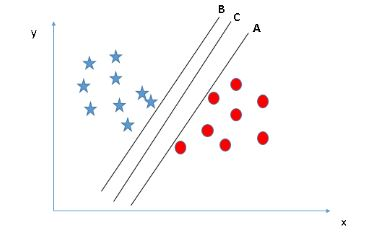
\includegraphics[scale=0.5]{Figures/svm13.png}
                \caption[Identify the right hyper-plane 2]{Identify the right hyper-plane 2}
                \label{fig:my_label}
            \end{figure}
        \item Here, maximizing the distances between nearest data point (either class) and hyper-plane will help us to decide the right hyper-plane. This distance is called as Margin. Let’s look at the below snapshot:
            \begin{figure}[h!]
                \centering
                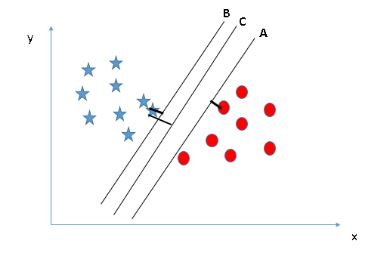
\includegraphics[scale=0.5]{Figures/svm14.png}
                \caption[Identify the right hyper-plane 2.1]{Identify the right hyper-plane 2.1}
                \label{fig:my_label}
            \end{figure}
        Above, we can see that the margin for hyper-plane C is high as compared to both A and B. Hence, the name of the right hyper-plane as C. Another lightning reason for selecting the hyper-plane with higher margin is robustness. If we select a hyper-plane having low margin then there is high chance of miss-classification.
        \item Identify the right hyper-plane (Scenario-3): Here use the rules as discussed in previous section to identify the right hyper-plane.
            \begin{figure}[h!]
                \centering
                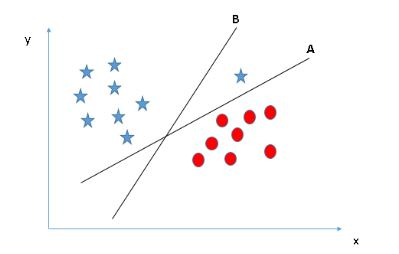
\includegraphics[scale=0.5]{Figures/svm15.png}
                \caption[Identify the right hyper-plane 3]{Identify the right hyper-plane 3}
                \label{fig:my_label}
            \end{figure}
        Some of us may have selected the hyper-plane B as it has higher margin compared to A. But, here is the catch, SVM selects the hyper-plane which classifies the classes accurately prior to maximizing margin. Here, hyper-plane B has a classification error and A has classified all correctly. Therefore, the right hyper-plane is A.
        
    \end{enumerate}

   
   \underline{The advantages of using SVM are listed as follows}:
   
   \begin{enumerate}
       \item SVM include high accuracy, elegant mathematical tractability, and direct geometric interpretation.
       \item It has few tunable parameters.
       \item Training often involves convex optimization. Hence, solutions are global and usually unique, thus avoiding the convergence to local minima exhibited by other statistical learning systems, such as neural networks.
   \end{enumerate}
   
\subsection{Decision Tree}

  Decision Trees are a type of Supervised Machine Learning (that is explain what the input is and the corresponding output is in the training data) where the data is continuously split according to a certain parameter. The tree can be explained by two entities, namely decision nodes and leaves. The leaves are the decisions or the final outcomes. And the decision nodes are where the data is split.
  
    \begin{figure}[h!]  
        \centering
        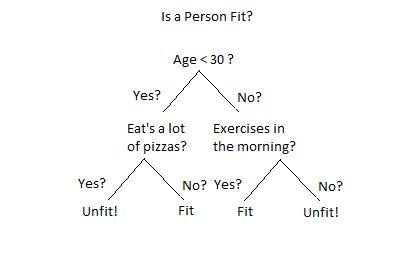
\includegraphics[scale=0.7]{Figures/decisiontree1.JPG}
        \caption{Decision Tree}[Decision Tree]
        \label{fig:my_label}
    \end{figure}
   
   An example of a decision tree can be explained using above binary tree. If you want to predict whether a person is fit given their information like age, eating habit, and physical activity, etc. The decision nodes here are questions like ‘What’s the age?’, ‘Does he exercise?’, ‘Does he eat a lot of pizzas’? And the leaves, which are outcomes like either ‘fit’, or ‘unfit’. In this case this was a binary classification problem (yes no type problem).
   
   There are two main types of Decision Trees:
   
   \begin{enumerate}
       \item Classification trees (Yes/No types):
       What we have seen above is an example of classification tree, where the outcome was a variable like ‘fit’ or ‘unfit’. Here the decision variable is Categorical.
       \item Regression trees (Continuous data types):
       Here the decision or the outcome variable is Continuous, e.g. a number like 123.
   \end{enumerate}
   
   \underline{Advantages}:
   
   \begin{enumerate}
       \item Minimum requirement of data cleaning
       \item Method is Non Parametric
       \item Can be used in Data exploration
       \item Constraint of Data type not present
       \item Can be easily Understandable
   \end{enumerate}
   
  \underline{Disadvantages}:
  
  \begin{enumerate}
      \item Over fitting
      \item Not fit for continuous variables
  \end{enumerate}
    
   \textbf{\underline{Working}}:
    
    The best algorithm to construct decision tree  is ID3 Algorithm. ID3 Stands for Iterative Dichotomiser 3.
    
    \textbf{Entropy}
    
    Entropy, also called as Shannon Entropy is denoted by H(S) for a finite set S, is the measure of the amount of uncertainty or randomness in data.
    
    
    \begin{figure}[h!]
        \centering
        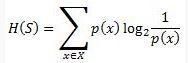
\includegraphics[scale=0.8]{Figures/a1.png}
    \end{figure}
   
   Intuitively, it tells us about the predictability of a certain event. Example, consider a coin toss whose probability of heads is 0.5 and probability of tails is 0.5. Here the entropy is the highest possible, since there’s no way of determining what the outcome might be. Alternatively, consider a coin which has heads on both the sides, the entropy of such an event can be predicted perfectly since we know beforehand that it’ll always be heads. In other words, this event has no randomness hence it’s entropy is zero.
   
   \textbf{Information Gain}

   Information gain is also called as Kullback-Leibler divergence denoted by IG(S,A) for a set S is the effective change in entropy after deciding on a particular attribute A. It measures the relative change in entropy with respect to the independent variables.
  
   
   \begin{figure}[h!]
        \centering
        
\includegraphics[scale=0.8]{Figures/a2.png}
   \end{figure}
  
   Alternatively,
   
   \begin{figure}[h!]
       \centering
         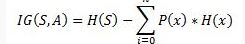
\includegraphics[scale=0.8]{Figures/a3.png}
   \end{figure}
  
   where IG(S, A) is the information gain by applying feature A. H(S) is the Entropy of the entire set, while the second term calculates the Entropy after applying the feature A, where P(x) is the probability of event x.
  
\subsection{Naive Bayes}
  
  Naive Bayes is a machine learning algorithm for classification problems. It is based on Bayes’ probability theorem. It is primarily used for text classification which involves high dimensional training data sets. A few examples are spam filtration, sentimental analysis, and classifying news articles.
  The Naive Bayes algorithm is called "naive" because it makes the assumption that the occurrence of a certain feature is independant of the occurance of other feature. 
  
  A Naive Bayes Classifier is a supervised machine-learning algorithm that uses the Bayes’ Theorem, which assumes that features are statistically independent. The theorem relies on the naive assumption that input variables are independent of each other, i.e. there is no way to know anything about other variables when given an additional variable. Regardless of this assumption, it has proven itself to be a classifier with good results.
  
  Naive Bayes Classifiers rely on the Bayes’ Theorem, which is based on conditional probability or in simple terms, the likelihood that an event (A) will happen given that another event (B) has already happened. Essentially, the theorem allows a hypothesis to be updated each time new evidence is introduced. The equation below expresses Bayes’ Theorem in the language of probability:
  
    \begin{figure}[h!]
        \centering
        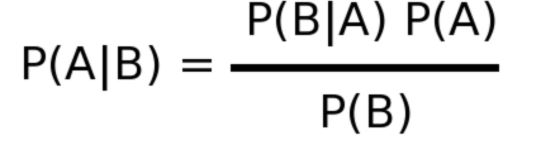
\includegraphics[scale=0.5]{Figures/eq2.png}
    \end{figure}

\subsection{MLP}
   
    The multi-layer perceptron is a feed forward neural network consisting of an input layer of nodes, followed by two or more layers of perceptron, the last of which is the output layer. The layers between the input layer and output layer are referred to as hidden layers. It has a lot of successful applications in solving complex problems in the real world, consisting of non-linear decision boundaries.
    
    MLP does not have any cycles and the output depends only
   on the input samples therefore it is named feed forward. It depends on supervised learning. Learning process conducted by changing the connection weights after handling each piece of data, based on the amount of error in the output target compared with the expected result. The main goal of a learning step is to reduce the error through improving the current values of the weight associated with each edge. Due to the process of backward changing of the weights, it’s called as backpropagation. 
   
   \begin{figure}[h!]
       \centering
       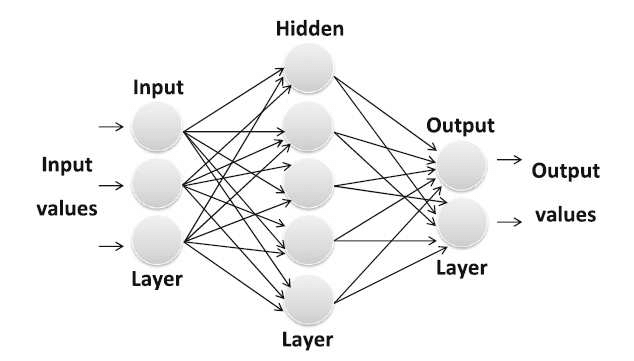
\includegraphics[scale=0.5]{Figures/MLP.png}
       \caption[MLP classifier]{MLP classifier}
       \label{fig:my_label}
   \end{figure}
   
   
\subsection{Logistic Regression}

  Logistic regression is a classification algorithm used to assign observations to a discrete set of classes. Unlike linear regression which outputs continuous number values, logistic regression transforms its output using the logistic sigmoid function to return a probability value which can then be mapped to two or more discrete classes.
  
  Logistic Regression could help use predict whether the student passed or failed. Logistic regression predictions are discrete (only specific values or categories are allowed). We can also view probability scores underlying the model’s classifications.
  
       \underline{Types of Logistic Regression}:
       \begin{enumerate}
           \item Binary: Target variable can have only 2 possible types: “0” or “1” which may represent “win” vs “loss”, “pass” vs “fail”, “dead” vs “alive”, etc.
           \item Multinomial: Target variable can have only 2 possible types: “0” or “1” which may represent “win” vs “loss”, “pass” vs “fail”, “dead” vs “alive”, etc.
           \item Ordinal: It deals with target variables with ordered categories. For example, a test score can be categorized as:“very poor”, “poor”, “good”, “very good”. Here, each category can be given a score like 0, 1, 2, 3.
       \end{enumerate}
       
\newpage
\section{Proposed CNN Model}

In machine learning, a convolutional neural network (CNN, or ConvNet) is a class of deep, feed-forward artificial neural networks that have successfully been applied to analyzing visual imagery. CNNs use a variation of multilayer perceptron designed to require minimal preprocessing. They are also known as shift invariant or space invariant artificial neural networks (SIANN), based on their shared-weights architecture and translation in variance characteristics. CNN was used to achieve some breakthrough results and win well-known contests. The application of convolutional layers consists in convolving a signal or an image with kernels to obtain feature maps. So, a unit in a feature map is connected to the previous layer through the weights of the kernels. The weights of the kernels are adapted during the training phase by back propagation, in order to enhance certain characteristics of the input. Since the kernels are shared among all units of the same feature maps, convolutional layers have fewer weights to train than dense FC layers, making CNN easier to train and less prone to overfitting. Moreover, since the same kernel is convolved over the entire image, the same feature is detected independently of the locating—translation in variance. By using kernels, information of the neighborhood is taken into account, which is a useful source of context information. Usually, a non-linear activation function is applied to the output of each neural unit.
If we stack several convolutional layers, the extracted features become more abstract with the increasing depth. The first layers enhance features such as edges, which are aggregated in the following layers as motifs, parts, or objects. The following concepts are important in the context of CNN:

\begin{enumerate}
    \item Initialization: It is important to achieve convergence. To achieve faster convergence Xavier initialization. With this, the activations and the gradients are maintained at controlled levels, otherwise, back-propagated gradients could vanish or explode.
    \item Pooling: It combines spatially nearby features in the feature maps. This combination of possibly redundant features makes the representation more compact and invariant to small image changes, such as insignificant details; it also decreases the computational load of the next stages. To join features, it is more common to use max-pooling or average-pooling.
    \item Regularization: It is used to reduce overfitting. Dropout is applied in the FC layers. In each training step, it removes nodes from the network with probability. In this way, it forces all nodes of the FC layers to learn better representations of the data, preventing nodes from co-adapting to each other. At test time, all nodes are used. Dropout can be seen as an ensemble of different networks and a form of bagging since each network is trained with a portion of the training data.
    \item Data Augmentation: It can be used to increase the size of training sets and reduce overfitting. Since the class of the patch is obtained by the central voxel, we restricted the data augmentation to rotating operations. Some authors also consider image translations, but for segmentation, this could result in attributing a wrong class to the patch. Proposed method increased our data set during training by generating new patches through the rotation of the original patch. In our proposal, we used angles a multiple of 90, although another alternative will be evaluated.
    \item Loss Function: It is the function to be minimized during training. We used the Categorical Cross-entropy
    7) Architecture: We aim at a reliable segmentation method; however, brain tumors present large variability in intra- tumoral structures, which makes the segmentation a challenging problem. To reduce such complexity, we designed a CNN and tuned the intensity normalization transformation for each tumor grade—LGG and HGG.
    Performance
    
    We used the U-Net Architecture for the above steps. The architecture is described as follows:
    
    \begin{figure}[h!]
       \centering
       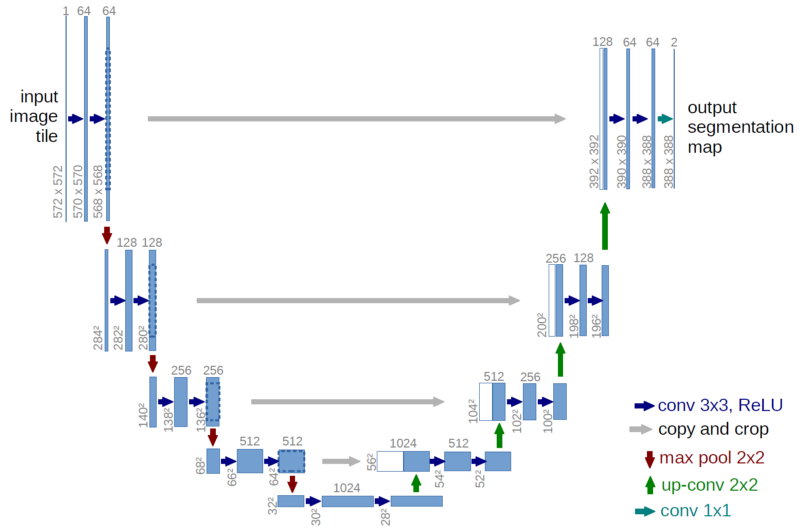
\includegraphics[scale=0.5]{Figures/unet.png}
       \caption[UNet Architecture]{UNet Architecture}
       \label{fig:UNet Architecture}
   \end{figure}
   
   The architecture looks like a ‘U’ which justifies its name. This architecture consists of three sections: The contraction, The bottleneck, and the expansion section. The contraction section is made of many contraction blocks. Each block takes an input applies two 3X3 convolution layers followed by a 2X2 max pooling. The number of kernels or feature maps after each block doubles so that architecture can learn the complex structures effectively. The bottommost layer mediates between the contraction layer and the expansion layer. It uses two 3X3 CNN layers followed by 2X2 up convolution layer.

    But the heart of this architecture lies in the expansion section. Similar to contraction layer, it also consists of several expansion blocks. Each block passes the input to two 3X3 CNN layers followed by a 2X2 upsampling layer. Also after each block number of feature maps used by convolutional layer get half to maintain symmetry. However, every time the input is also get appended by feature maps of the corresponding contraction layer. This action would ensure that the features that are learned while contracting the image will be used to reconstruct it. The number of expansion blocks is as same as the number of contraction block. After that, the resultant mapping passes through another 3X3 CNN layer with the number of feature maps equal to the number of segments desired.
    
    \subsection{Loss calculation in UNet}
    UNet uses a rather novel loss weighting scheme for each pixel such that there is a higher weight at the border of segmented objects. This loss weighting scheme helped the U-Net model segment cells in biomedical images in a discontinuous fashion such that individual cells may be easily identified within the binary segmentation map.

    First of all pixel-wise softmax applied on the resultant image which is followed by cross-entropy loss function. So we are classifying each pixel into one of the classes. The idea is that even in segmentation every pixel have to lie in some category and we just need to make sure that they do. So we just converted a segmentation problem into a multi-class classification one and it performed very well as compared to the traditional loss functions.

    \subsection{Training}
    The input images and their corresponding segmentation maps are used to train the network with the stochastic gradient descent implementation of Caffe [6]. Due to the unpadded convolutions, the output image is smaller than the input by a constant border width. To minimize the overhead and make maximum use of the GPU memory, we favor large input tiles over a large batch size and hence reduce the batch to a single image. Accordingly we use a high momentum (0.99) such that a large number of the previously seen training samples determine the update in the current optimization step.
    
    \subsection{Data Augmentation}
    Data augmentation is essential to teach the network the desired invariance and robustness properties, when only few training samples are available. In case of microscopical images we primarily need shift and rotation invariance as well as robustness to deformations and gray value variations. Especially random elas- tic deformations of the training samples seem to be the key concept to train a segmentation network with very few annotated images. We generate smooth deformations using random displacement vectors on a coarse 3 by 3 grid. The displacements are sampled from a Gaussian distribution with 10 pixels standard deviation. Per-pixel displacements are then computed using bicubic interpola- tion. Drop-out layers at the end of the contracting path perform further implicit data augmentation.

    
\end{enumerate}



      
  
% Chapter 5

\chapter{Result and Discussion}% Main chapter title

\label{Chapter5} % For referencing the chapter elsewhere, use \ref{Chapter} 

\lhead{Chapter 5. \emph{ Result and Discussion }} % This is for the header on each page - perhaps a shortened title

%--------------------------------------------------------------------------------
The dataset we used is originally from BraTS(Brain Tumor Segmentation) dataset.It consists of 

\begin{itemize}
    \item HGG: This folder contains brain images of 220 Patients.There is a
       different folder for each patient. There are 5 different MRI images
       for each Patient. The 5 different images are T1, T2, T1C, FLAIR and
       OT(Ground truth of tumor Segmentation). All these image files
       are stored in .mha format.
       \item LGG - This folder contains brain images of 54 Patients.There is a
       different folder for each patient. There are 5 different MRI images
       for each Patient. The 5 different images are T1, T2, T1C, FLAIR and
       OT(Ground truth of tumor Segmentation). All these image files
       are stored in .mha format.
\end{itemize}
The dataset can be downloaded from: \emph{https://braintumorsegmentation.org/}

\section{Performance of different Machine Learning Algorithms}
We have applied different classification techniques on the above mentioned dataset.  We have allotted 70\% of the data for training and 30\% for testing.  The different classification techniques we used are MLP,  Support Vector Machine, K Nearest Neighbour and Random Forest Classifier.  The results of these classifiers are discussed below:

\begin{table}[h!]
    \centering
    \begin{tabular}{|p{2cm}|l|l|}
    \hline
    \textbf{Classifier} & \textbf{Accuracy}  & \textbf{Loss} \\
    \hline
    MLP & 90.05\% & 0.34\% \\
    \hline
    KNN & 88.55\%  & 0.43\% \\
    \hline
    SVM & 90.04\% & 0.39\% \\
    \hline
    Random Forest & 88.05\% & 0.41\% \\
    \hline
    \end{tabular}
    \caption{Accuracy of different Classifiers}
    \label{tab:my_label}
\end{table}
\newpage
\section{Training of CNN Model}

We used BraTS 2018 dataset for training of our CNN Model. We have divided the dataset into two parts: 70\% for training purpose and 30\% for Validation/testing purpose.

\begin{table}[h!]
    \centering
    \begin{tabular}{|p{2cm}|p{2cm}|}
         \hline
         \textbf{Parameters} & \textbf{Range of values} \\
         \hline
         Number of Epochs & 15 \\
         \hline
         Accuracy & 0.9945 \\
         \hline
         Loss & 0.3777 \\
         \hline
         Best Epoch & 8 \\
         \hline
         Elapsed Time & 39s 222ms/step \\
         \hline
    \end{tabular}
    \caption{Training parameters and values of CNN}
    \label{tab:my_label}
\end{table}

In this model, on using Sigmoid activation function in the dense layer, we achieve an accuracy of 100\% which shows that the network might suffering from a case of overfitness and may work inefficiently for a larger dataset. \\ Thus, we have used ReLU activation function for all convolution layers for which we have achieved 99.45\% accuracy which is an acceptable score for this network.


Plots for the training and Validation are shown below:

 \begin{figure}[htbp]
	    \centering
		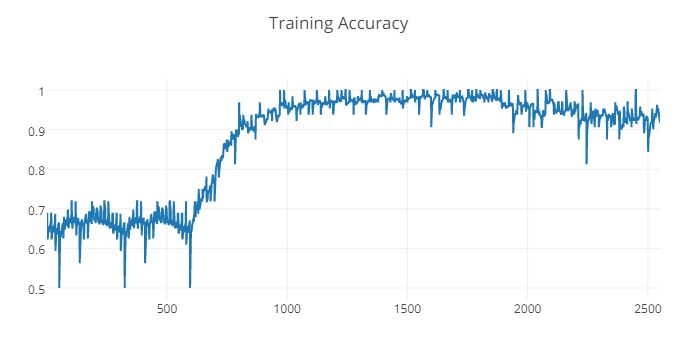
\includegraphics[scale=0.5]{Figures/trainingAccuracy(him).JPG}
		%\rule{10em}{0.5pt}
	    \caption[Training Accuracy]{Training Accuracy}
	    \label{fig:trainccuracy}
        \end{figure}
        
        \begin{figure}[htbp]
	    \centering
		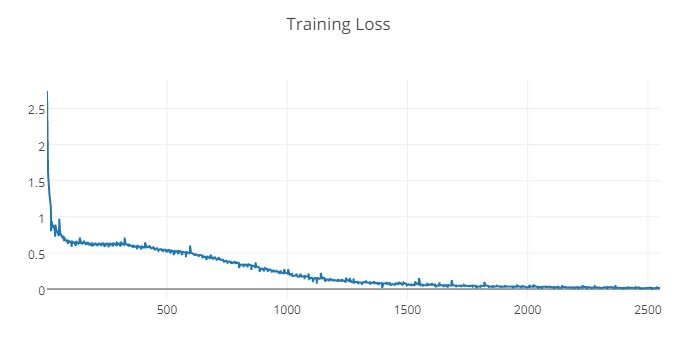
\includegraphics[scale=0.5]{Figures/trainingLoss(him).JPG}
		%\rule{10em}{0.5pt}
	    \caption[Training Loss]{Training Loss}
	    \label{fig:trainloss}
        \end{figure}
        
        
        
        \begin{figure}[htbp]
	    \centering
		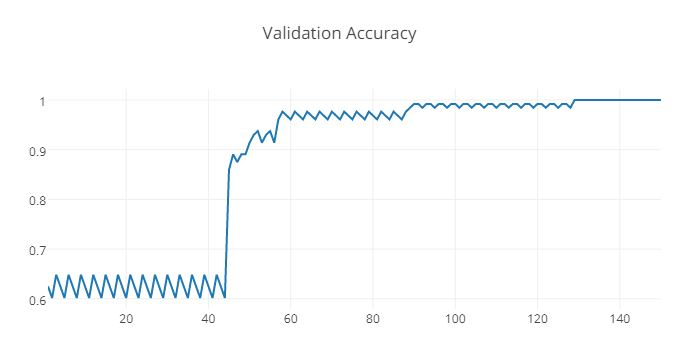
\includegraphics[scale=0.5]{Figures/validationAccuracy(him).JPG}
		%\rule{10em}{0.5pt}
	    \caption[Validation Accuracy]{Validation Accuracy}
	    \label{fig:valacc}
        \end{figure}
        
        \begin{figure}[htbp]
	    \centering
		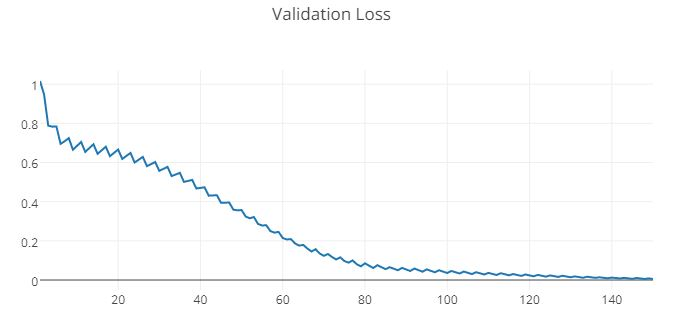
\includegraphics[scale=0.5]{Figures/validationLoss(him).JPG}
		%\rule{10em}{0.5pt}
	    \caption[Validation Loss]{Validation Loss}
	    \label{fig:valloss}
        \end{figure}
        
        \begin{figure}[htbp]
	    \centering
		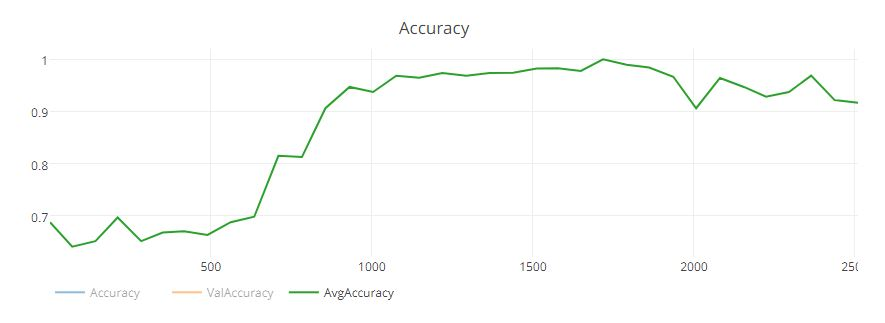
\includegraphics[scale=0.5]{Figures/avgAccuracy(him).JPG}
		%\rule{10em}{0.5pt}
	    \caption[Average Accuracy]{Average Accuracy}
	    \label{fig:avgacc}
        \end{figure}
        
        \begin{figure}[htbp]
	    \centering
		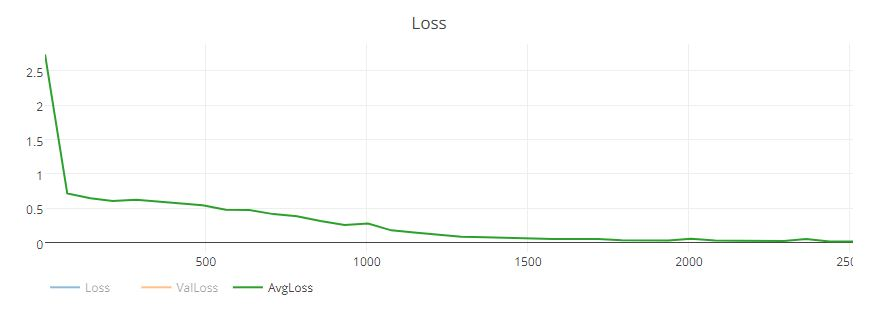
\includegraphics[scale=0.5]{Figures/avgLoss(him).JPG}
		%\rule{10em}{0.5pt}
	    \caption[Average Loss]{Average Loss}
	    \label{fig:avgloss}
        \end{figure} 
% Chapter 6 

\chapter{Conclusion} % Main chapter title

\label{Chapter6} % For referencing the chapter elsewhere, use \ref{Chapter6} 

\lhead{Chapter 6. \emph{ Conclusion }} % This is for the header on each page - perhaps a shortened title

%--------------------------------------------------------------------------------
  
  In this study, using MR images of the brain, we segmented brain tissues into normal tissues such as white matter, gray matter, cerebrospinal fluid (background), and tumor-infected tissues.. We used preprocessing to improve the signal-to-noise ratio and to eliminate the effect of unwanted noise. We used a skull stripping algorithm based on threshold technique to improve the skull stripping performance. Furthermore, we used U-Net architecture with Fully Convolutional Neural Networks to classify the tumor stage by analyzing feature vectors and area of the tumor. In this study, we investigated texture based and histogram based features with a commonly recognized classifier for the classification of brain tumor from MR brain images.
  
  From the experimental results performed on the different images, it is clear that the analysis for the brain tumor detection is fast and accurate when compared with the manual detection performed by radiologists or clinical experts. The various performance factors also indicate that the proposed algorithm provides better result by improving certain parameters such as mean, MSE, PSNR, accuracy, sensitivity, specificity, and dice coefficient. Our experimental results show that the proposed approach can aid in the accurate and timely detection of brain tumor along with the identification of its exact location. Thus, the proposed approach is significant for brain tumor detection from MR images.
    Dataset consist of 220 3d images of tumor and non-tumor.
    In this study, a model has been proposed for the efficient tumor detection of brain MR images. Following steps are adopted for detection:
    \begin{enumerate}
        \item Step 1: Taking input image.
        \item Step 2: Filter image.
        \item Step 3: Segmentation of MR image by gray scaled technique.
        \item Step 4: Then apply classification technique of deep neural network to detect the tumor from brain MR images. Accuracy of the classification is 99\%.
        \item Step 5: Last task is to compute the area of the detected image by using algorithm.
    \end{enumerate}
    
    
    
   
     
%% Chapter Template

\chapter{Machine Learning} % Main chapter title

\label{Chapter7} % Change X to a consecutive number; for referencing this chapter elsewhere, use \ref{ChapterX}

\lhead{Chapter 2. \emph{Machine Learning}} % Change X to a consecutive number; this is for the header on each page - perhaps a shortened title

%----------------------------------------------------------------------------------------
%	SECTION 1
%----------------------------------------------------------------------------------------

\section{Definition}

Machine Learning is the field of study that gives computers the capability to learn without being explicitly programmed. ML is one of the most exciting technologies that one would have ever come across. As it is evident from the name, it gives the computer that which makes it more similar to humans: The ability to learn. Machine learning is actively being used today, perhaps in many more places than one would expect.

\begin{itemize}
\item Traditional Programming: Data and program is run on the computer to produce the output.
\item Machine Learning: Data and output is run on the computer to create a program. This program can be used in traditional programming.
\end{itemize}
\begin{figure}[htbp]
    \centering
	    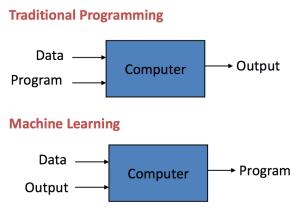
\includegraphics[scale=0.5]{Figures/tl_ml.png}
		    %\rule{10em}{0.5pt}
        \caption[Traditional programming vs Machine Learning]{Traditional programming vs Machine Learning}
	    \label{fig:Traditional programming vs Machine Learning}
\end{figure}
 Machine learning is like farming or gardening. Seeds is the algorithms, nutrients is the data, the gardener is you and plants is the programs.
\clearpage
\section{Types of Machine Learning}

At a high-level, machine learning is simply the study of teaching a computer program or algorithm how to progressively improve upon a set task that it is given. On the research-side of things, machine learning can be viewed through the lens of theoretical and mathematical modeling of how this process works. However, more practically it is the study of how to build applications that exhibit this iterative improvement. There are many ways to frame this idea, but largely there are three major recognized categories:
\begin{enumerate}
    \item Supervised learning
    \item Unsupervised learning
    \item Reinforcement learning
\end{enumerate}

\begin{figure}[htbp]
    \centering
	    \includegraphics[scale=0.3]{Figures/ml_types.jpg}
		    %\rule{10em}{0.5pt}
        \caption[Types of Machine Learning]{Types of Machine Learning}
	    \label{fig:Traditional programming vs Machine Learning}
\end{figure}

\subsection{Supervised Learning}

Supervised learning is the most popular paradigm for machine learning. It is the easiest to understand and the simplest to implement.\\
Given data in the form of examples with labels, we can feed a learning algorithm these example-label pairs one by one, allowing the algorithm to predict the label for each example, and giving it feedback as to whether it predicted the right answer or not. Over time, the algorithm will learn to approximate the exact nature of the relationship between examples and their labels. When fully-trained, the supervised learning algorithm will be able to observe a new, never-before-seen example and predict a good label for it.

\begin{figure}[htbp]
    \centering
	    \includegraphics[scale=0.4]{Figures/supervised.png}
		    %\rule{10em}{0.5pt}
        \caption[Supervised Learning]{Supervised Learning}
	    \label{fig:Supervised Learning}
\end{figure}

Supervised Learning uses two types of techniques:

\begin{itemize}
    \item Classification:
        Classification is the process of predicting the class of given data points. Classes are sometimes called as targets/ labels or categories. Classification predictive modeling is the task of approximating a mapping function (f) from input variables (X) to discrete output variables (y).

        For example, spam detection in email service providers can be identified as a classification problem. This is s binary classification since there are only 2 classes as spam and not spam. A classifier utilizes some training data to understand how given input variables relate to the class. In this case, known spam and non-spam emails have to be used as the training data. When the classifier is trained accurately, it can be used to detect an unknown email.

        Classification belongs to the category of supervised learning where the targets also provided with the input data. There are many applications in classification in many domains such as in credit approval, medical diagnosis, target marketing etc.

        There are two types of learners in classification as lazy learners and eager learners.
        \begin{enumerate}
            \item Lazy learners: Lazy learners simply store the training data and wait until a testing data appear. When it does, classification is conducted based on the most related data in the stored training data. Compared to eager learners, lazy learners have less training time but more time in predicting.

            \textit {Ex. k-nearest neighbor, Case-based reasoning}
    
            \item Eager learners: Eager learners construct a classification model based on the given training data before receiving data for classification. It must be able to commit to a single hypothesis that covers the entire instance space. Due to the model construction, eager learners take a long time for train and less time to predict.

            \textit{Ex. Decision Tree, Naive Bayes, Artificial Neural Networks}
    
        \end{enumerate}
        Classification Algorithms:\\
        There is a lot of classification algorithms available now but it is not possible to conclude which one is superior to other. It depends on the application and nature of available data set. For example, if the classes are linearly separable, the linear classifiers like Logistic regression, Fisher’s linear discriminant can outperform sophisticated models and vice versa.
        \begin{itemize}
            \item Decision Tree:
                
                Decision tree builds classification or regression models in the form of a tree structure. It utilizes an if-then rule set which is mutually exclusive and exhaustive for classification. The rules are learned sequentially using the training data one at a time. Each time a rule is learned, the tuples covered by the rules are removed. This process is continued on the training set until meeting a termination condition.
            
            \begin{figure}[htbp]
                \centering
	            \includegraphics[scale=0.3]{Figures/decision_tree.png}
		        %\rule{10em}{0.5pt}
                \caption[Decision Tree]{Decision Tree}
	            \label{fig:Decision Tree}
                \end{figure}

                The tree is constructed in a top-down recursive divide-and-conquer manner. All the attributes should be categorical. Otherwise, they should be discretized in advance. Attributes in the top of the tree have more impact towards in the classification and they are identified using the information gain concept.

                A decision tree can be easily over-fitted generating too many branches and may reflect anomalies due to noise or outliers. An over-fitted model has a very poor performance on the unseen data even though it gives an impressive performance on training data. This can be avoided by pre-pruning which halts tree construction early or post-pruning which removes branches from the fully grown tree.

        \item Naive Bayes:
                Naive Bayes is a probabilistic classifier inspired by the Bayes theorem under a simple assumption which is the attributes are conditionally independent.\\
                    \begin{figure}[htbp]
                        \centering
	                    \includegraphics[scale=0.5]{Figures/naive_bayes.png}
		                %\rule{10em}{0.5pt}
                        \caption[Naive Bayes]{Naive Bayes}
	                    \label{fig:Naive Bayes}
                    \end{figure}
                The classification is conducted by deriving the maximum posterior which is the maximal P(Ci|X) with the above assumption applying to Bayes theorem. This assumption greatly reduces the computational cost by only counting the class distribution. Even though the assumption is not valid in most cases since the attributes are dependent, surprisingly Naive Bayes has able to perform impressively.

                Naive Bayes is a very simple algorithm to implement and good results have obtained in most cases. It can be easily scalable to larger datasets since it takes linear time, rather than by expensive iterative approximation as used for many other types of classifiers.

                Naive Bayes can suffer from a problem called the zero probability problem. When the conditional probability is zero for a particular attribute, it fails to give a valid prediction. This needs to be fixed explicitly using a Laplacian estimator.
                
        \item Artificial Neural Networks:
                Artificial Neural Network is a set of connected input/output units where each connection has a weight associated with it started by psychologists and neurobiologists to develop and test computational analogs of neurons. During the learning phase, the network learns by adjusting the weights so as to be able to predict the correct class label of the input tuples.

                \begin{figure}[htbp]
                    \centering
	                \includegraphics[scale=0.3]{Figures/ann.jpeg}
		            %\rule{10em}{0.5pt}
                    \caption[Artificial Neural Network Design]{Artificial Neural Network Design}
	                \label{fig:Naive Bayes}
                \end{figure}
                
                There are many network architectures available now like Feed-forward, Convolutional, Recurrent etc. The appropriate architecture depends on the application of the model. For most cases feed-forward models give reasonably accurate results and especially for image processing applications, convolutional networks perform better.

                There can be multiple hidden layers in the model depending on the complexity of the function which is going to be mapped by the model. Having more hidden layers will enable to model complex relationships such as deep neural networks.

                However, when there are many hidden layers, it takes a lot of time to train and adjust wights. The other disadvantage of is the poor interpretability of model compared to other models like Decision Trees due to the unknown symbolic meaning behind the learned weights.

                But Artificial Neural Networks have performed impressively in most of the real world applications. It is high tolerance to noisy data and able to classify untrained patterns. Usually, Artificial Neural Networks perform better with continuous-valued inputs and outputs.

        \item k-Nearest Neighbor (KNN):
                \begin{figure}[htbp]
                    \centering
	                \includegraphics[scale=0.3]{Figures/knn.png}
		            %\rule{10em}{0.5pt}
                    \caption[k-Nearest Neighbor]{k-Nearest Neighbor}
	                \label{fig:Naive Bayes}
                \end{figure}
        
                k-Nearest Neighbor is a lazy learning algorithm which stores all instances correspond to training data points in n-dimensional space. When an unknown discrete data is received, it analyzes the closest k number of instances saved (nearest neighbors)and returns the most common class as the prediction and for real-valued data it returns the mean of k nearest neighbors.

                In the distance-weighted nearest neighbor algorithm, it weights the contribution of each of the k neighbors according to their distance using the following query giving greater weight to the closest neighbors.

                \begin{figure}[htbp]
                    \centering
	                \includegraphics[scale=0.5]{Figures/knn2.png}
		            %\rule{10em}{0.5pt}
                    \caption[Distance calculating query]{Distance calculating query}
	                \label{fig:Naive Bayes}
                \end{figure}
        \end{itemize}
    \item Regression:
                \begin{figure}[htbp]
                    \centering
	                \includegraphics[scale=0.4]{Figures/linear_r.png}
		            %\rule{10em}{0.5pt}
                    \caption[Distance calculating query]{Distance calculating query}
	                \label{fig:Naive Bayes}
                \end{figure}
    
        Simple linear regression is a type of regression analysis where the number of independent variables is one and there is a linear relationship between the independent(x) and dependent(y) variable. The red line in the above graph is referred to as the best fit straight line. Based on the given data points, we try to plot a line that models the points the best. The line can be modelled based on the linear equation shown below.
    
                \begin{figure}[htbp]
                    \centering
	                \includegraphics[scale=0.8]{Figures/linear_r1.png}
		            %\rule{10em}{0.5pt}
                \end{figure}
                
        The motive of the linear regression algorithm is to find the best values for a0 and a1. Before moving on to the algorithm, let’s have a look at two important concepts you must know to better understand linear regression.
        
        \clearpage
        Cost Function: The cost function helps us to figure out the best possible values for a0 and a1 which would provide the best fit line for the data points. Since we want the best values for a0 and a1, we convert this search problem into a minimization problem where we would like to minimize the error between the predicted value and the actual value.
        
                \begin{figure}[htbp]
                    \centering
	                \includegraphics[scale=0.5]{Figures/costfn.png}
		            %\rule{10em}{0.5pt}
		            \caption[Minimization and Cost Function]{Minimization and Cost Function}
	                \label{fig:Minimization and Cost Function}
                \end{figure}
                
        We choose the above function to minimize. The difference between the predicted values and ground truth measures the error difference. We square the error difference and sum over all data points and divide that value by the total number of data points. This provides the average squared error over all the data points. Therefore, this cost function is also known as the Mean Squared Error(MSE) function. Now, using this MSE function we are going to change the values of a0 and a1 such that the MSE value settles at the minima.
        
        Gradient Descent: The next important concept needed to understand linear regression is gradient descent. Gradient descent is a method of updating a0 and a1 to reduce the cost function(MSE). The idea is that we start with some values for a0 and a1 and then we change these values iteratively to reduce the cost. Gradient descent helps us on how to change the values.

                \begin{figure}[htbp]
                    \centering
	                \includegraphics[scale=0.4]{Figures/lrate.png}
		            %\rule{10em}{0.5pt}
		            \caption[Learning Rate]{Learning Rate}
	                \label{fig:Learning Rate}
                \end{figure}
        To draw an analogy, imagine a pit in the shape of U and you are standing at the topmost point in the pit and your objective is to reach the bottom of the pit. There is a catch, you can only take a discrete number of steps to reach the bottom. If you decide to take one step at a time you would eventually reach the bottom of the pit but this would take a longer time. If you choose to take longer steps each time, you would reach sooner but, there is a chance that you could overshoot the bottom of the pit and not exactly at the bottom. In the gradient descent algorithm, the number of steps you take is the learning rate. This decides on how fast the algorithm converges to the minima.
    
\end{itemize}
\subsection{Unsupervised Learning}
    Unsupervised Learning is a class of Machine Learning techniques to find the patterns in data. The data given to unsupervised algorithm are not labelled, which means only the input variables(X) are given with no corresponding output variables. In unsupervised learning, the algorithms are left to themselves to discover interesting structures in the data. 

%----------------------------------------------------------------------------------------
%	THESIS CONTENT - APPENDICES
%----------------------------------------------------------------------------------------

\addtocontents{toc}{\vspace{2em}} % Add a gap in the Contents, for aesthetics

\appendix % Cue to tell LaTeX that the following 'chapters' are Appendices

% Include the appendices of the thesis as separate files from the Appendices folder
% Uncomment the lines as you write the Appendices

%% Appendix A

\chapter{Appendix Title Here} % Main appendix title

\label{AppendixA} % For referencing this appendix elsewhere, use \ref{AppendixA}

\lhead{Appendix A. \emph{Appendix Title Here}} % This is for the header on each page - perhaps a shortened title

Write your Appendix content here.
%\input{Appendices/AppendixB}
%\input{Appendices/AppendixC}

\addtocontents{toc}{\vspace{2em}} % Add a gap in the Contents, for aesthetics

\backmatter

%----------------------------------------------------------------------------------------
%	BIBLIOGRAPHY
%----------------------------------------------------------------------------------------

\label{Bibliography}

% \bibliography{References}
%\addcontentsline{toc}{chapter}{\large{Bibliography}}
\begin{thebibliography}{99}

\bibitem{ref1}Binu Thomas and P K Nizar Banu, "Brain tumor segmentation and detection using MRI images" ,International Journal of Mechanical Engineering and Technology (IJMET) Volume 9, Issue 5, May 2018.

\bibitem{ref2}Hussna Elnoor Mohammed Abdalla and M. Y. Esmail,"Brain Tumor Detection by using Artificial Neural Network ",  International Conference on Computer, Control, Electrical, and Electronics Engineering (ICCCEEE),2018.

\bibitem{ref3}Hao Dong ,Guang Yang, Fangde Liu, Yuanhan Mo, Yike Guo ,"  Automatic Brain Tumor Detection and Segmentation Using U-Net Based Fully Convolutional Networks", IJRET: International Journal of Research in Engineering and Technology, eISSN: 2319-1163 | pISSN: 2321-7308 , 2015.

\bibitem{ref4}Shubhangi S. Veer and Pradeep M. Patil,"Brain tumor classification using Artificial neural network on MRI images",International Journal of Advanced Research in  Electrical, Electronics and Instrumentation Engineering, ISSN (Print)  : 2320 – 3765,ISSN (Online): 2278 – 8875,Vol. 3, Issue 9, September 2014.

\bibitem{ref5}Aqhsa Q. Syed and K. Narayanan."Detection of Tumor in MRI Images Using Artificial Neural Networks",IJCSI International Journal of Computer Science Issues, Vol. 9, Issue 3, No 3, May 2012,ISSN (Online): 1694-0814 .

\bibitem{ref6}Nitish Zulpe and Vrushsen Pawar
,"GLCM Textural Features for Brain Tumor Classification",IJCSI International Journal of Computer Science Issues, Vol. 9, Issue 3, No 3, May 2012,ISSN (Online): 1694-0814.

\end{thebibliography}


\end{document}